% LaTeX source for ``Introduction to Computer Science (Java/Pi Edition)''
% Copyright (c) 2015- David S. Read, All Rights Reserved

\chapter{Raspberry Pi Labs}


\section{A Platform for Experimentation and Learning}

\index{Raspberry Pi}

In the early days of home computing the machines were very basic and packaged software was limited to 
some simple games and very basic office tools. Many computers were targeted at hobbyists who would 
write their own programs. There was no Internet full of information and media to consume,
so the computer was a device for active experimentation rather than passive entertainment.

Over the years computers have become more sophisticated, expensive and central to many household operations
(such as paying bills) while the Internet grew up and provided a nearly inexhaustible amount
of content and functionality to use and explore. Computers transitioned from experimental
workshops for hobbyists to a common appliance, leveraged by all family members for a variety
of purposes.

The Raspberry Pi\footnote{Another small computing device good for experimentation is the Arduino} was created
by several individuals who work in the computer science field and felt that having an affordable
computer for basic experimentation would be of interest to the general public. It appears they were correct
given the increasing popularity of the Pi, including its use in production environments.

This chapter will introduce you to the Raspberry Pi 3 while providing a series of lab exercises for you
to complete. The labs are intended to meet two goals: 

\begin{itemize}
	
\item Have some fun building simple circuits and interacting with them using programs you write.

\item Reinforce the principles of object oriented programming by associating physical objects (LEDs and buttons)
with virtual objects (instances of classes) and seeing how the attributes and behaviors in the
virtual environments manifest in the physical world.

\end{itemize}

\section{Introducing the Raspberry Pi 3}

\begin{figure}[H]
	\centering
	%	\begin{mdframed}
	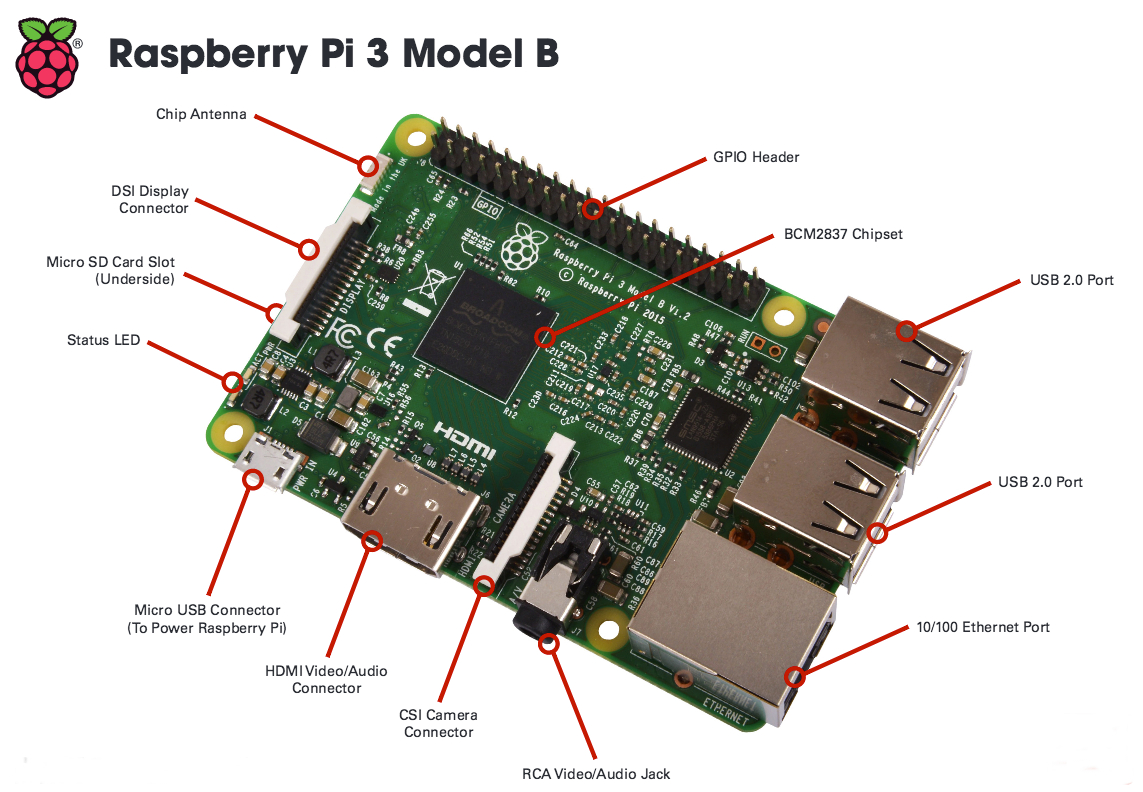
\includegraphics[height=3.50in]{pi_images/Raspi-3-Layout.jpg}
	%	\end{mdframed}
	\caption{The Raspberry Pi 3 with key components labeled}
	\label{fig:raspberrypi3}
\end{figure}

Hereafter I'll generally refer to the Raspberry Pi as the Pi.

The Pi is a great environment for learning about computing devices and programming. It has several key 
advantages over programming on a general computer system:

\begin{itemize}
	\item it is a relatively inexpensive full-featured computing device
	\item it is capable of running a variety of commodity software development tools
	\item it provides access to input and output signals via its General Purpose Input/Output (GPIO) connector
\end{itemize}

The first two advantages are straightforward. The GPIO interface deserves a little more definition.

\section{GPIO - General Purpose Input/Output}

\index{GPIO}

We often interact with computers using screens, keyboards and mice. Sometimes we use other input devices
such as scanners and drawing tablets. We can output information to printers or other computers across a network.
Often that is the limit of our direct computer interactions. However, inside the computer there are
a variety of electrical signals being used to communicate between the computer's components. These core components, which
we discussed in chapter 0, include the CPU, main memory, disk drives and network cards.

Typically we don't have any easy way to interface directly with these types of signals. For example, many computers
have a light which indicates when the disk drive is being accessed. Generally we don't have access to that
electrical signal, we just see the light flickering.

The Pi's J8 GPIO interface allows us to attach devices to the Pi and use them for input and output. For example
we can connect an LED to a GPIO pin and then write a program that turns the LED on and off. Similarly we
can connect a button to another GPIO pin and use the button as a signal for a program to take a certain
action when the button is pressed.

Figure~\ref{fig:j8header} is a close-up of the GPIO J8 40-pin interface that depicts several pin numbers (these are \textbf{\textit{not}} the GPIO numbers, which we'll see shortly). The pins are simply numbered sequentially:

\begin{figure}[H]
	\centering
	%	\begin{mdframed}
	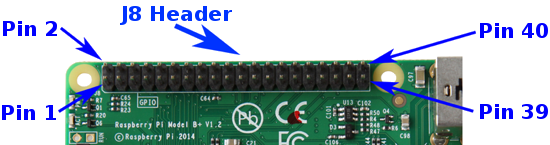
\includegraphics[height=1.30in]{pi_images/j8header-photo-transparentbg.png}
	%	\end{mdframed}
	\caption{Raspberry Pi 3's J8 Header with several pins labeled}
	\label{fig:j8header}
\end{figure}

To allow our programs to interface with the pins we need a way to identify which physical pins we want to 
control from within our program. The Pi uses a numbering scheme where the controllable pins are assigned
a GPIO number. Unfortunately different versions of the Pi have used different GPIO numbering schemes. 

To
deal with this numbering confusion, the Java library we will be using, known as Pi4J\footnote{Short for \textbf{Pi \textit{for} Java}. You can read more about this library at \url{http://pi4j.com/}}, assigns consistent GPIO numbers to the
pins regardless of which Pi device we are using. 

\pagebreak

Figure~\ref{fig:pi4jgpio} depicts the GPIO numbers assigned by the Pi4J library. We will use these numbers throughout the chapter. You'll want to keep 
track of this figure for quick reference when you are building the lab circuits.

\begin{figure}[H]
	\centering
	%	\begin{mdframed}
	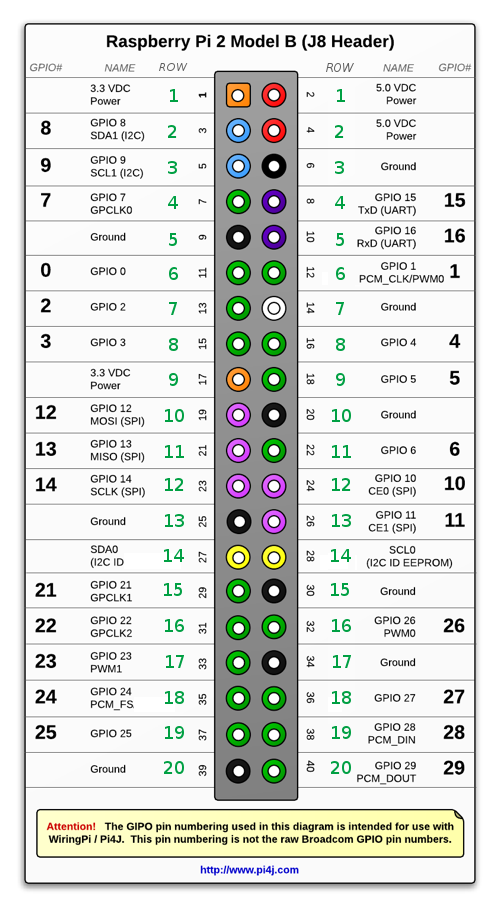
\includegraphics[height=6.0in]{pi_images/j8header-2b-dsr-flat.png}
	%	\end{mdframed}
	\caption{The Pi's J8 pin and row numbers with the Pi4J GPIO numbering}
	\label{fig:pi4jgpio}
\end{figure}

The bold numbers at the extreme right and left of the diagram are the GPIO numbers. The numbers in green give the row number of the pin (useful when we are describing the wiring for a lab project since they line up with the row numbers printed on the breadboard). The small vertically-oriented (sideways) numbers are the physical pin numbers which we generally won't be concerned with.

\pagebreak

\section{Breadboards - Easy Wiring}

\index{breadboard}

In order to create our lab project circuits, we will use
a breadboard which allows us to easily connect different
electrical devices to the Pi without worrying about soldering. A breadboard has a set of electrically-connected
holes into which we insert jumper wires, LEDs,
buttons, etc.

Figure~\ref{fig:breadboard} is a picture of the breadboard we will be using for the labs:

\begin{figure}[H]
	\centering
	%	\begin{mdframed}
	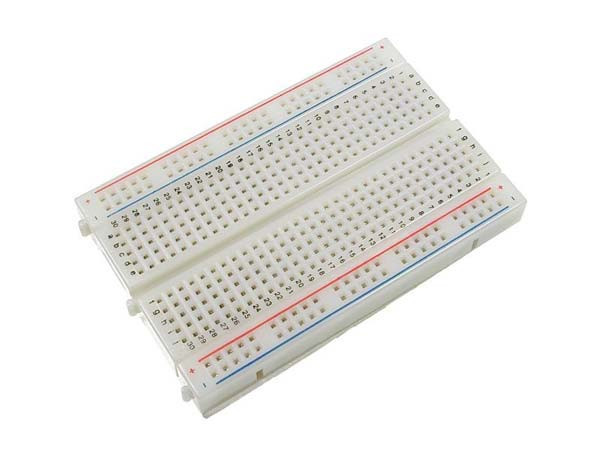
\includegraphics[height=2in]{pi_images/half-size-breadboard-600x600_grande.jpg}
	%	\end{mdframed}
	\caption{Standard half-size breadboard}
	\label{fig:breadboard}
\end{figure}

Note that there are 14 columns of holes. The first and last two columns are special (marked with + and -). The center set of 10 columns are labeled a-j in two groups, a-e and f-j. There are 30 rows of holes available for columns a-j.

Let's consider how the breadboard is wired internally. The connection points for the first and last two columns (labeled + and -) are electrically connected by column. The connection points in the columns labeled a-e and the ones in columns f-j are connected horizontally in groups of 5. For example a connection to point a1 is connected to holes b1, c1, d1 and e1. Similarly f1 is connected to g1, h1, i1 and j1.

These images below attempt to clarify how the holes are tied together:

%\beforefig
%\centerline{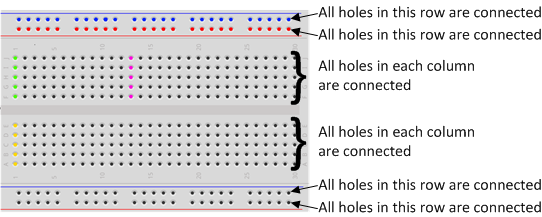
\includegraphics[height=2.00in]{pi_images/Breadboard_Remarked_grande.png}}
%\afterfig

\iffalse % comment out images displayed one above the other

\beforefig
\centerline{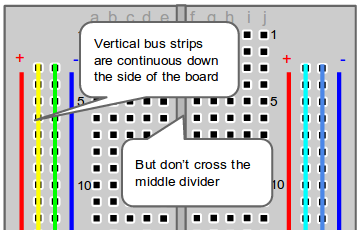
\includegraphics[height=2.0in]{pi_images/verticalpower.png}}
\afterfig

\beforefig
\centerline{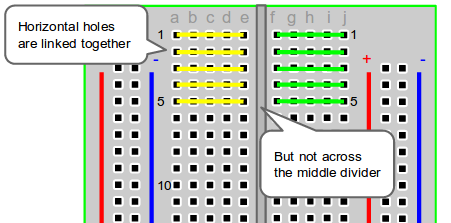
\includegraphics[height=2.0in]{pi_images/horizontal-rows.png}}
\afterfig

\fi % end of skipping images

\begin{tabular}{p{0.4\textwidth} p{0.3\textwidth}}
	\vspace{0pt} 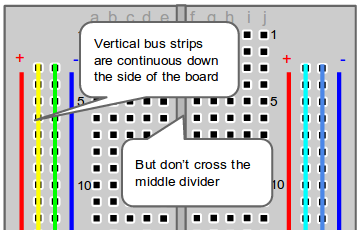
\includegraphics[height=1.4in]{pi_images/verticalpower.png} &
	\vspace{0pt} 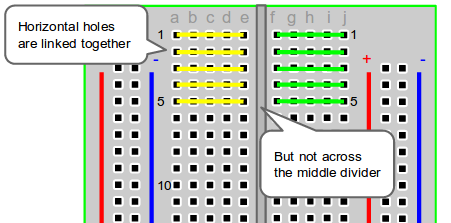
\includegraphics[height=1.4in]{pi_images/horizontal-rows.png}
\end{tabular}



This layout will make more sense once you complete the first lab 
and put together your initial set of components.

\section{Connecting the Pi and a Breadboard}

It may have occurred to you that there is no way to directly attach the breadboard to the Pi. For that we need two more pieces of equipment: a breakout board and ribbon cable.

A breakout board\footnote{Also called a cobbler breakout} provides a way to connect the 40 pins from the J8 GPIO interface to separate sets of holes on the breadboard. A ribbon cable then allows us to connect the breakout board to the Pi.

Figure~\ref{fig:piwithbreadboard} shows the entire setup, connecting the Pi to the ribbon cable, which attaches to the breakout board which is installed on the breadboard. This is the basic workbench we will be using for our Pi labs.

\begin{figure}[H]
	\centering
	%	\begin{mdframed}
	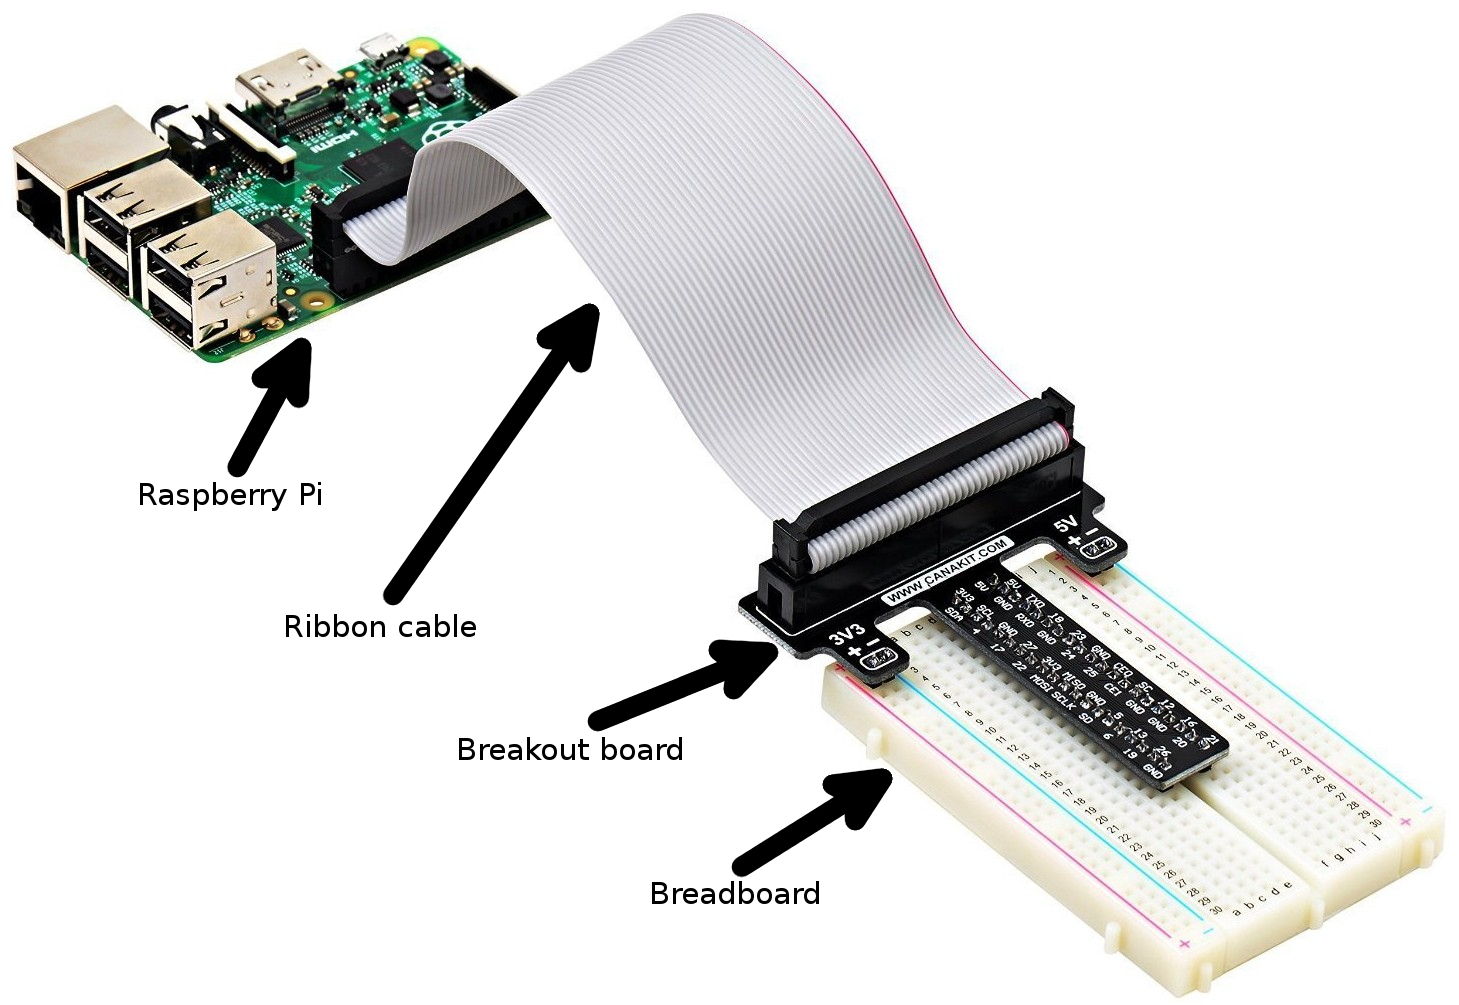
\includegraphics[height=2.5in]{pi_images/breadboard-cobbler-pi.jpg}
	%	\end{mdframed}
	\caption{Raspberry Pi, ribbon cable, breakout board and breadboard}
	\label{fig:piwithbreadboard}
\end{figure}

\section{Electronics - keeping it basic}

This book is not intended to make you an electrical engineer. Each lab will clearly spell out all of the 
connections you need to make in order to setup the 
breadboard for the specific assignment. Your job will be
to write programs. In this case the programs will control
(or be controlled by) devices attached to the Pi via the breadboard.

\pagebreak

The basic components you will be working with are:

\begin{enumerate}
\item \textbf{Jumper cables}

\index{jumper cable}
\index{breadboard!jumper cable}

\beforefig
\centerline{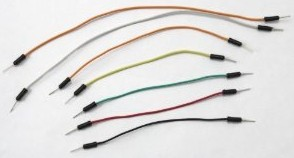
\includegraphics[height=1.50in]{pi_images/breadboard-jumper-cables.jpg}}
\afterfig

Jumper cables have a pin at each end that are easily inserted into the breadboard holes. The cables are used to connect one set of holes to another set of holes. For example, when we need to connect an LED to a GPIO pin we will insert one end of a jumper cable into the same row as the GPIO pin and insert the other end of the jumper into a hole in the same row with the LED's wire.

\item \textbf{Resistors}

\beforefig
\centerline{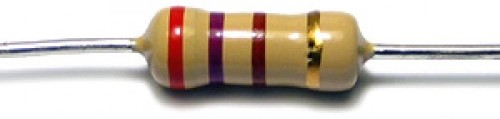
\includegraphics[height=0.50in]{pi_images/resistor3-500x500.jpg}}
\afterfig

A resistor, as its name implies, resists the flow of electricity through a circuit. In our case we want to be sure that we do not damage the Pi or our LEDs with too high a current flow.

The resistors have two connecting wires whose orientation doesn't matter. When we list two holes on the breadboard for the resistor's wires to be inserted into, you can insert either end of the resistor into either hole.

\item \textbf{Buttons}

\index{button}
\index{breadboard!button}

\beforefig
\centerline{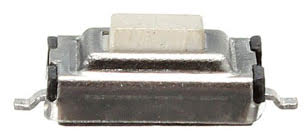
\includegraphics[height=0.70in]{pi_images/button_large.jpg}}
\afterfig

The buttons we will use are known as momentary contact buttons. This means that they only make contact (complete a circuit) while being held down. Our programs can then respond to the button being pressed when the Pi detects that a circuit has been completed by the button. Here is a diagram of how the switch is wired.

\beforefig
\centerline{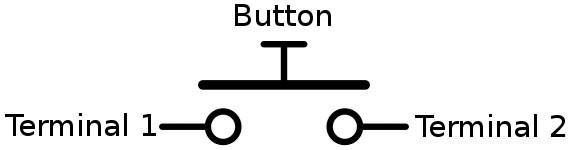
\includegraphics[height=0.70in]{pi_images/button_schematic.png}}
\afterfig

Like resistors, each button has two connection points and their orientation does not matter. When we list two holes on the breadboard for the button's terminals to be inserted into, you can insert either end of the button into either hole.

\iffalse % Ignoring this information for the 4 connection buttons

\beforefig
\centerline{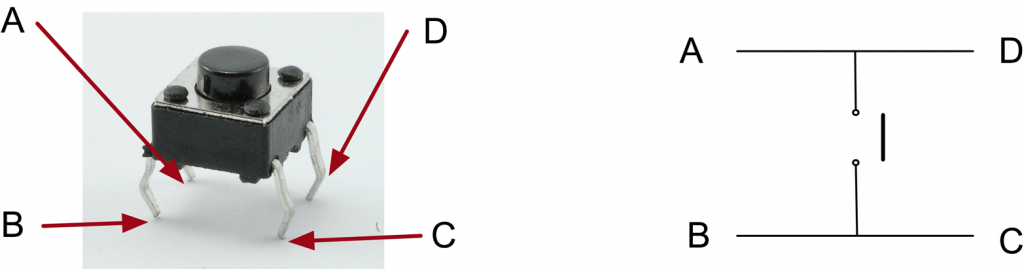
\includegraphics[height=1.00in]{pi_images/Push-Switch-fs8-1024x269.png}}
\afterfig

The buttons we will use are known as momentary contact buttons. This means that they only make contact (complete a circuit) while being held down. Our programs can then respond to the button being pressed when the Pi detects that a circuit has been completed by the button. Above is a picture of a button with a diagram of how the switch is wired.

Don't worry about the A-B-C-D labeling yet. We'll formally work through connecting the switch in the first lab to use one. It turns out the orientation of the button will matter when we place it on the breadboard.

\textbf{\underline{Take note that the orientation of buttons matters}}. Looking at the bottom of the buttons you'll note that they have four contacts. In one direction the contacts are closer together than in the other. Looking at the diagram above, the A-D and B-C contacts are more widely spaced than the A-B and C-D contacts.

For our labs, \textbf{when inserting the buttons into the breadboard you will need to place them so that the more widely spaced contacts are arranged on opposite sides of the breadboard's center line}. That is, A-B goes on one side of the center line and C-D go on the other. \textit{If you're unsure about their placement, check with your instructor.}

\fi % End of ignored section discussing the 4 contact buttons

\item \textbf{LEDs}

\index{LED}
\index{breadboard!LED}

\beforefig
\centerline{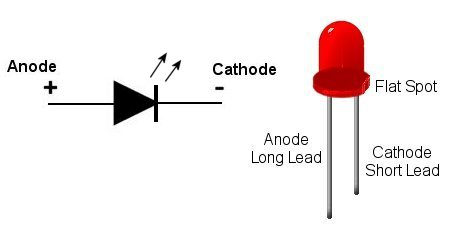
\includegraphics[height=1.50in]{pi_images/led_2.jpg}}
\afterfig

The acronym LED stands for Light Emitting Diode. A key term is diode. A diode is sensitive to the direction of electrical current flow. There is a right way and wrong way to connect one.

The anode end must tie to the positive side of the circuit while the cathode end must tie to the negative side. You can identify the anode on the LED since it has a longer connector wire. 

If the wire lengths are too close to differentiate you can also look for a flat spot on one side of the LED. The wire nearest the flat spot will be the cathode.


\end{enumerate}

Those are the only components we will work with for this set of labs. They extend our keyboard and screen with new ways to interact with the computer, pressing a button to provide input and lighting an LED to provide output.

\section{PiLib - classes for components}

\index{PiLib}
\index{library!PiLib}

We've toured through the hardware we'll be using. Now we need to describe the software that will allow us to turn on LEDs and detect button presses.

\textbf{\underline{Widget Control}} \newline

The library, called PiLib, is comprised of several classes that are used to represent the physical components. Developers often call such components widgets. The base class in PiLib for interacting with
physical components is Widget. This class is abstract so you won't be creating any instances of it.

Each Widget subclass will represent a physical component such as an LED or button. Since any physical component must be connected to a GPIO pin in order to be accessible from the Pi, the Widget class has an attribute representing the GPIO number (as depicted in the earlier Pi4J numbering diagram).

Below is an overview of the specific Widget subclasses that you will be using. The first time each one is used in a lab we will go into more detail.

Also, note that there is complete JavaDoc for PiLib. It can be found with the library itself as well as at:  \url{https://monead.com/iot/PiLibClient/}.

\index{PiLib!JavaDoc location}

The four classes of interest are:

\begin{enumerate}
	\item \textbf{Widget} \newline
	This represents any widget. Each of the classes listed below are subclasses of Widget. The Widget class has a few special static methods including \textbf{\texttt{gpioReset()}} which removes old GPIO pin mappings.
	
\index{Widget class}
\index{PiLib!Widget class}
\index{gpioReset() method}
\index{Widget.gpioReset() method}
\index{PiLib!gpioReset() method}

	You'll normally want to call that at the beginning of your program to be sure there aren't any old GPIO pin mappings configured. You call the method by simply including the statement \textbf{\texttt{Widget.gpioReset();}} in your program before creating your mappings. You may also call it at the end of your program to remove mappings and leave the environment in a clean state. 
	
	The Widget class also defines the static methods \textbf{\texttt{turnOffAllLeds()}}, \textbf{\texttt{turnOnAllLedsSolid()}} and \textbf{\texttt{turnOnAllLedsBlink()}} which are convenience methods to quickly set all the LEDs to a specific mode.

\index{turnOffAllLeds() method}
\index{Widget.turnOffAllLeds() method}
\index{PiLib!turnOffAllLeds() method}
\index{turnOnAllLedsSolid() method}
\index{Widget.turnOnAllLedsSolid() method}
\index{PiLib!turnOnAllLedsSolid() method}
\index{turnOnAllLedsBlink() method}
\index{Widget.turnOnAllLedsBlink() method}
\index{PiLib!turnOnAllLedsBlink() method}
	
	For controlling \texttt{BinaryLed} instances (see below) the \textbf{\texttt{Widget.setBinaryValue()}} method takes an \texttt{int} parameter which is the value you want displayed by the \texttt{BinaryLed} instances.
	
\index{BinaryLed class}
\index{PiLib!BinaryLed class}

	If you review the JavaDoc for the Widget class you will see that it also contains a method called \texttt{shutdown()}. You will rarely use this method since it shuts down the PiLibServer. \textit{You cannot make further use of the library methods (for instance you can't call methods on the Led instances) once the  \texttt{shutdown()} method is called until you restart the PiLibServer program.} 

	\item \textbf{Button} \newline
	This represents the operations and attributes that are allowed for a button. The operations are detecting that the button has been pressed, getting a count of times it has been pressed and resetting the button's counter.
	
	The three methods of interest provided by the Button class are \textbf{\texttt{getPressCount()}}, \textbf{\texttt{clearPressCount()}} and \textbf{\texttt{waitForPress()}}. See the JavaDoc for details.

\index{Button class}
\index{PiLib!Button class}
\index{getPressCount() method}
\index{Button.getPressCount() method}
\index{PiLib!Button.getPressCount() method}
\index{clearPressCount() method}
\index{Button.clearPressCount() method}
\index{PiLib!Button.clearPressCount() method}
\index{waitForPress() method}
\index{Button.waitForPress() method}
\index{PiLib!Button.waitForPress() method}
	
	\item \textbf{Led} \newline
	This represents the operations that are allowed for an LED. The operations include turning the LED off, turning it on and making it blink. There are no additional attributes associated with an LED.
	
	The three methods of interest provided by the Led class are \textbf{\texttt{turnOff()}}, \textbf{\texttt{turnOnSolid()}} and \textbf{\texttt{turnOnBlink()}}. See the JavaDoc for details.
					
\index{Led class}
\index{PiLib!Led class}
\index{turnOff() method}
\index{Led.turnOff() method}
\index{PiLib!Led.turnOff() method}
\index{turnOnSolid() method}
\index{Led.turnOnSolid() method}
\index{PiLib!Led.turnOnSolid() method}
\index{turnOnBlink() method}
\index{Led.turnOnBlink() method}
\index{PiLib!Led.turnOnBlink() method}
	
	\item \textbf{BinaryLed} \newline
	This represents an LED that is being used in a group
	with other LEDs as a way to represent binary numbers. Don't worry about binary if you aren't familiar with it. We'll cover it in a later lab. The \texttt{Widget.setBinaryValue()} method (described above) is used to make displaying of binary numbers easy.
	
	\texttt{BinaryLed} is a subclass of \texttt{Led} meaning it inherits the \texttt{Led} class's methods \textbf{\texttt{turnOff()}}, \textbf{\texttt{turnOnSolid()}} and \textbf{\texttt{turnOnBlink()}}. See the PiLib JavaDoc for details.
					
\index{BinaryLed class}
\index{PiLib!BinaryLed class}
\index{turnOff() method}
\index{BinaryLed.turnOff() method}
\index{PiLib!BinaryLed.turnOff() method}
\index{turnOnSolid() method}
\index{BinaryLed.turnOnSolid() method}
\index{PiLib!BinaryLed.turnOnSolid() method}
\index{turnOnBlink() method}
\index{BinaryLed.turnOnBlink() method}
\index{PiLib!BinaryLed.turnOnBlink() method}
	
\end{enumerate}

The classes that you will use in your programs send commands to a server program. That program must be running on your Pi. The server, \textbf{PiLibServer}, needs special permissions in order to access the GPIO pins. See the section, \textbf{\textit{Starting the PiLib Server}} for information in using the PiLib server program.

\textbf{\underline{Utilities}} \newline

In addition to classes for controlling the widgets, PiLib has several utility methods to make working with the Pi and interacting with users a little simpler. Each of these methods is in the \textbf{\texttt{Utility}} class.

\begin{enumerate}
	\item \textbf{Collecting user input} \newline
	Many labs require our program to ask the user for information that must be supplied using the keyboard. Java makes it fairly easy to read input from the keyboard, however there is a redundant set of code that has to be written each time we want to get another piece of information.
	
	To simplify keyboard input, the \texttt{Utility} class contains the method \textbf{\texttt{readKeyboardLine()}}. The method waits for the user to type some characters and press the \textbf{Enter} key. Once the user presses \textbf{Enter} the method returns a \textbf{String} containing any characters the user typed prior to pressing \textbf{Enter}.
	
	Here is a simple program that asks the user to enter their name, gets the information from the keyboard and then prints his or her response on the screen.
	
\beforeverb
\begin{verbatim}
import us.daveread.raspberrypi.gpio.lib.Utility;

public class DemokeyboardInput {
 public static void main(String[] args) {
  String name;

  System.out.print("What is your name? ");
  name = Utility.readKeyboardLine();

  System.out.println("You replied with the name " + name);
 }
}\end{verbatim}
\afterverb

Here is an example of what this would look like when it is run:

\beforeverb
\begin{verbatim}
What is your name? Dave
You replied with the name Dave
\end{verbatim}
\afterverb


	\item \textbf{Pausing Program Execution} \newline
	When you are working with the LEDs you will often need to have your program pause so that the LED stays on or off for a defined period of time. For instance, if you wrote a program to turn on an LED, the LED would turn off as soon as the program ended. If you want to have the LED stay on for a couple of seconds before the program ends (turning off the LED) you need a way to pause the program.
	
	The \texttt{Utility} class contains the method \textbf{\texttt{pause()}} which will cause the program to stop executing statements for a defined period of time. You tell the \texttt{pause()} method how long to pause by passing the number of milliseconds to pause as a parameter.
	
	Here is an example of using the \texttt{pause()} method to print out the message, \textit{Hello World! Glad to meet you.} one word at a time. The amount of time the program pauses is different between different words.
	
	The program pauses for 1 second (1000 milliseconds) after printing \textit{Hello}. It pauses one half-second after printing \textit{World!} Looking at the code you can see the other pause lengths being used. Give the program a try to experience how the output will be presented.
	
\beforeverb
\begin{verbatim}
import us.daveread.raspberrypi.gpio.lib.Utility;

public class DemoPause {
 public static void main(String[] args) {
  System.out.println("Hello");
  Utility.pause(1000);
  System.out.println("World!");
  Utility.pause(500);
  System.out.println("Glad");
  Utility.pause(1500);
  System.out.println("to");
  Utility.pause(250);
  System.out.println("meet");
  Utility.pause(750);
  System.out.println("you.");
  Utility.pause(1250);    
 }
}\end{verbatim}
\afterverb
	
\end{enumerate}

\section{Starting the PiLibServer}

If you have not installed the PiLib server please see the section \textbf{\textit{Setup the PiLib Server}} on page \pageref{setupPiLibServer} in the \textit{Raspberry Pi Setup} appendix.

\index{PiLib}
\index{library!PiLib}
\index{PiLib!Server program}

Whenever you want to use the PiLib server program you will use a terminal (accessing your home directory) and type the following command:

\textbf{\texttt{\$ PiLibServerDist/runServerSudo.sh}}

\textit{Note that the} \texttt{\$} \textit{(dollar sign) is the terminal prompt.} You do not type the \texttt{\$}. Also, your terminal prompt may look different than a plain dollar sign.

This command starts the server. Your screen should contain a message similar to:

\texttt{2016-06-16 10:37:55,869 [us.daveread.raspberrypi.gpio.lib.server.PiLibServer] [main] (PiLibServer.java:45) WARN  us.daveread.raspberrypi.gpio.lib.server.PiLibServer  - PiLib service ready}

You must leave the terminal open (running) while working on your Pi Lab program. You may close the PiLib Server by selecting the terminal and typing \textbf{\texttt{[Ctrl]C}}. That is, hold the [Ctrl] key and press the letter \textbf{C}.

\section{PiLib Server Web Control}

The PiLib Server supports a web-based interface for three purposes:

\begin{enumerate}
	\item Client library control
	\item Viewing the current GPIO configuration
	\item Interacting with the GPIO configuration
\end{enumerate}

\textbf{\underline{View Current GPIO Configuration}}

If you want to view the current configuration, use the following address in your browser (note that the PiLib server must be running when you do this):

\textbf{\texttt{\url{http://localhost:5162/PiLib}}}

If you are not running a program that has setup GPIO mappings then you will see an empty page containing the message, \textit{No widgets have been created} (figure~\ref{fig:servernowidget}). Otherwise you will see a graphical representation for each mapped LED and button (figure~\ref{fig:serverwithwidget}).

\begin{figure}[H]
	\centering
%	\begin{mdframed}
	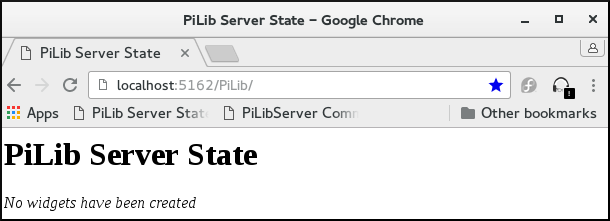
\includegraphics[height=1.50in]{pi_images/PiLibServerNoWidgets.png}
%	\end{mdframed}
	\caption{PiLib Server web page with no widgets}
	\label{fig:servernowidget}
\end{figure}

\begin{figure}[H]
	\centering
	%	\begin{mdframed}
	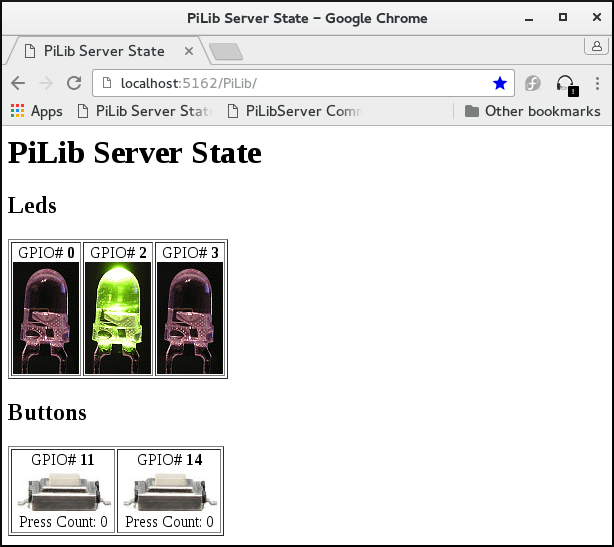
\includegraphics[height=1.8in]{pi_images/PiLibServerWithWidgets.png}
	%	\end{mdframed}
	\caption{PiLib Server web page with widgets configured}
	\label{fig:serverwithwidget}
\end{figure}

You may find this view helpful when building your Pi labs since you can see what GPIOs are configured for which components as well as seeing the state of the LEDs and interacting with the buttons. If you have your project setup and LEDs aren't lighting when expected or button presses aren't being detected, you can use this web page to see if the issue is with components on the breadboard or with the program.

\textbf{\underline{PiLib Server Test Web Page}}

If you want to test out a GPIO configuration without writing Java code you can setup several simple arrangements of components. The web URL for this is:

\textbf{\texttt{\url{http://localhost:5162/PiLib/test}}}

You may use this web page (figure~\ref{fig:servertestpage}) to modify the GPIO Configuration, mapping LEDs and buttons to GPIO numbers as well as clearing old mappings or even shutting-down the PiLib server. This page is intended for basic testing of the GPIO server. You will probably not find it particularly useful as you work through the Pi lab exercises.

\begin{figure}[H]
	\centering
	%	\begin{mdframed}
	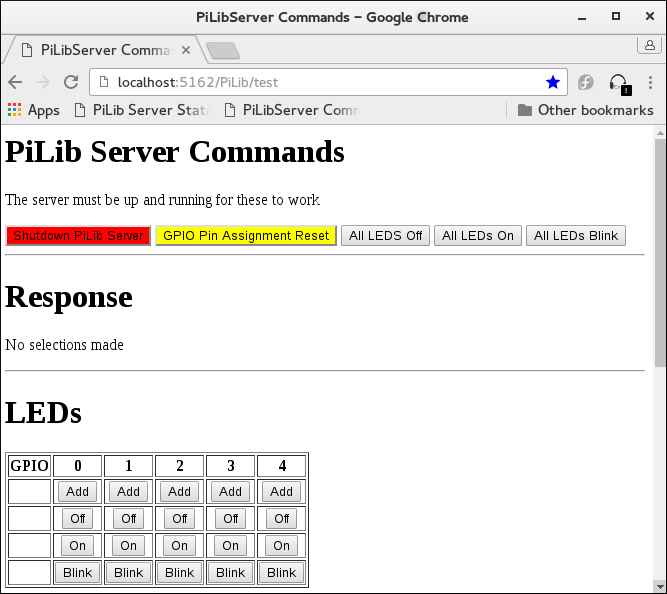
\includegraphics[height=1.8in]{pi_images/PiLibServerTestPage.png}
	%	\end{mdframed}
	\caption{PiLib Server test page (top of page)}
	\label{fig:servertestpage}
\end{figure}

\section{Wiring Tests}
\label{wiringTestDescription}
\index{PiLab Wiring Test}
\index{Wiring Test!PiLab}

\beforefig
\begin{wrapfigure}{r}{40mm}
	\centerline{
\includegraphics[height=1in]{images/approved-151676_960_720.png}}
\end{wrapfigure}
\afterfig

Every Pi Lab project includes a test program to check that all of the components are properly connected and working. The class file will always be called \textbf{\texttt{WiringTest.java}}.

For each lab, after wiring your breadboard and connecting it to your Pi, you should open the \textbf{\texttt{WiringTest}} program and run it. Depending on the components being used for your lab the program will exercise each one.

Generally it will turn on all the LEDs and then, if the lab uses buttons, it will have you press each button in sequence and report that the press was detected.

\beforefig
\begin{wrapfigure}{l}{40mm}
\centerline{
\includegraphics[height=1in]{images/exclamation-mark-red-md.png}}
\end{wrapfigure}
\afterfig

If one or more of the components aren't working when the \texttt{WiringTest} is run you will need to fix it. Here are the three most common issues I've seen which cause the test to fail:

\begin{itemize}
	\item The PiLib Server has not been started
	\item The ribbon cable connector which plugs into the Pi is loose or not aligned correctly
	\item The components are not wired correctly on the breadboard. A common wiring mistake is connecting resistors to the wrong power rail (such as connecting to 3V3+ when the connection should be to 3V3--).
\end{itemize}

Make sure that the \texttt{WiringTest} works before proceeding. Your own program won't work correctly if the test isn't working.

Now that we have discussed the PiLib client and server components as well as how to test our breadboard wiring, let's give it all a try with our first lab.


\clearpage

\section{Lab 1 - Part 1}

\textbf{Learning Goals}

\begin{enumerate}
	\item Create a working circuit with 1 LED controlled by a Java program running on the Pi
	\item Explore the Led class methods that allow us to control a physical LED
	\item Understand the relationship between virtual objects (instances of a class) and their physical counterparts
\end{enumerate}

\textbf{Overview}

You will use your breadboard to connect an LED to a GPIO pin. With this setup you will write a Java program which controls the LED. In a second part of the lab you will add a second LED and control both of them with a program.

\textbf{Breadboard Configuration}

\hfill

{\centering
\fbox{\begin{minipage}{300pt}
\textbf{\underline{WARNING:} NEVER connect or disconnect the breadboard's ribbon cable from your Raspberry Pi when the Pi is powered-up. NEVER change the wiring on your
breadboard when it is connected to your powered-up Raspberry Pi. \textit{You 
can do \underline{permanent damage} (including rendering your Pi unusable)
if you are changing connections while your Pi is running.} Your best bet is to do the wiring when your Pi is disconnected from a power source.}
\end{minipage}
}\par
}

\hfill

For each lab we'll provide two images of the configured breadboard. One image will depict the components using drawings that clearly show the connection points. The other image will be a photo of a completed breadboard to help you validate the overall arrangement of the components.

In addition to the images there will be a step by step set of connection instructions. If you are unsure of a connection, verify it with the instructor, TA or a classmate.

\pagebreak

\underline{Wiring Depiction}

\beforefig
\centerline{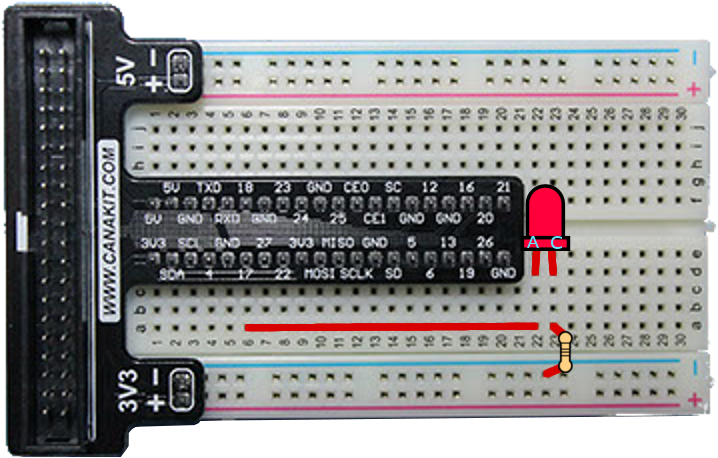
\includegraphics[height=2in]{pi_images/lab01images/PiLab01-1Light.png}}
\afterfig

\underline{Wiring Steps}

\textbf{Remember, your Pi must be disconnected from a power source while wiring the circuit.}

\begin{enumerate}
	\item Insert an LED anode (longer wire) into hole \textbf{d22}
	\item Insert the same LED's cathode into hole \textbf{d23}
	
	\item Insert a jumper from hole \textbf{a6} to hole \textbf{a22}
	
	\item Insert a resistor between hole \textbf{a23} and a \textbf{3V3--} (negative) hole adjacent to row 23.
	
	\item If your ribbon cable is not connected to the Pi and the breakout board, connect it now (making sure your Pi is disconnected from any power source)
\end{enumerate}

\underline{Completed Breadboard Picture}

\beforefig
\centerline{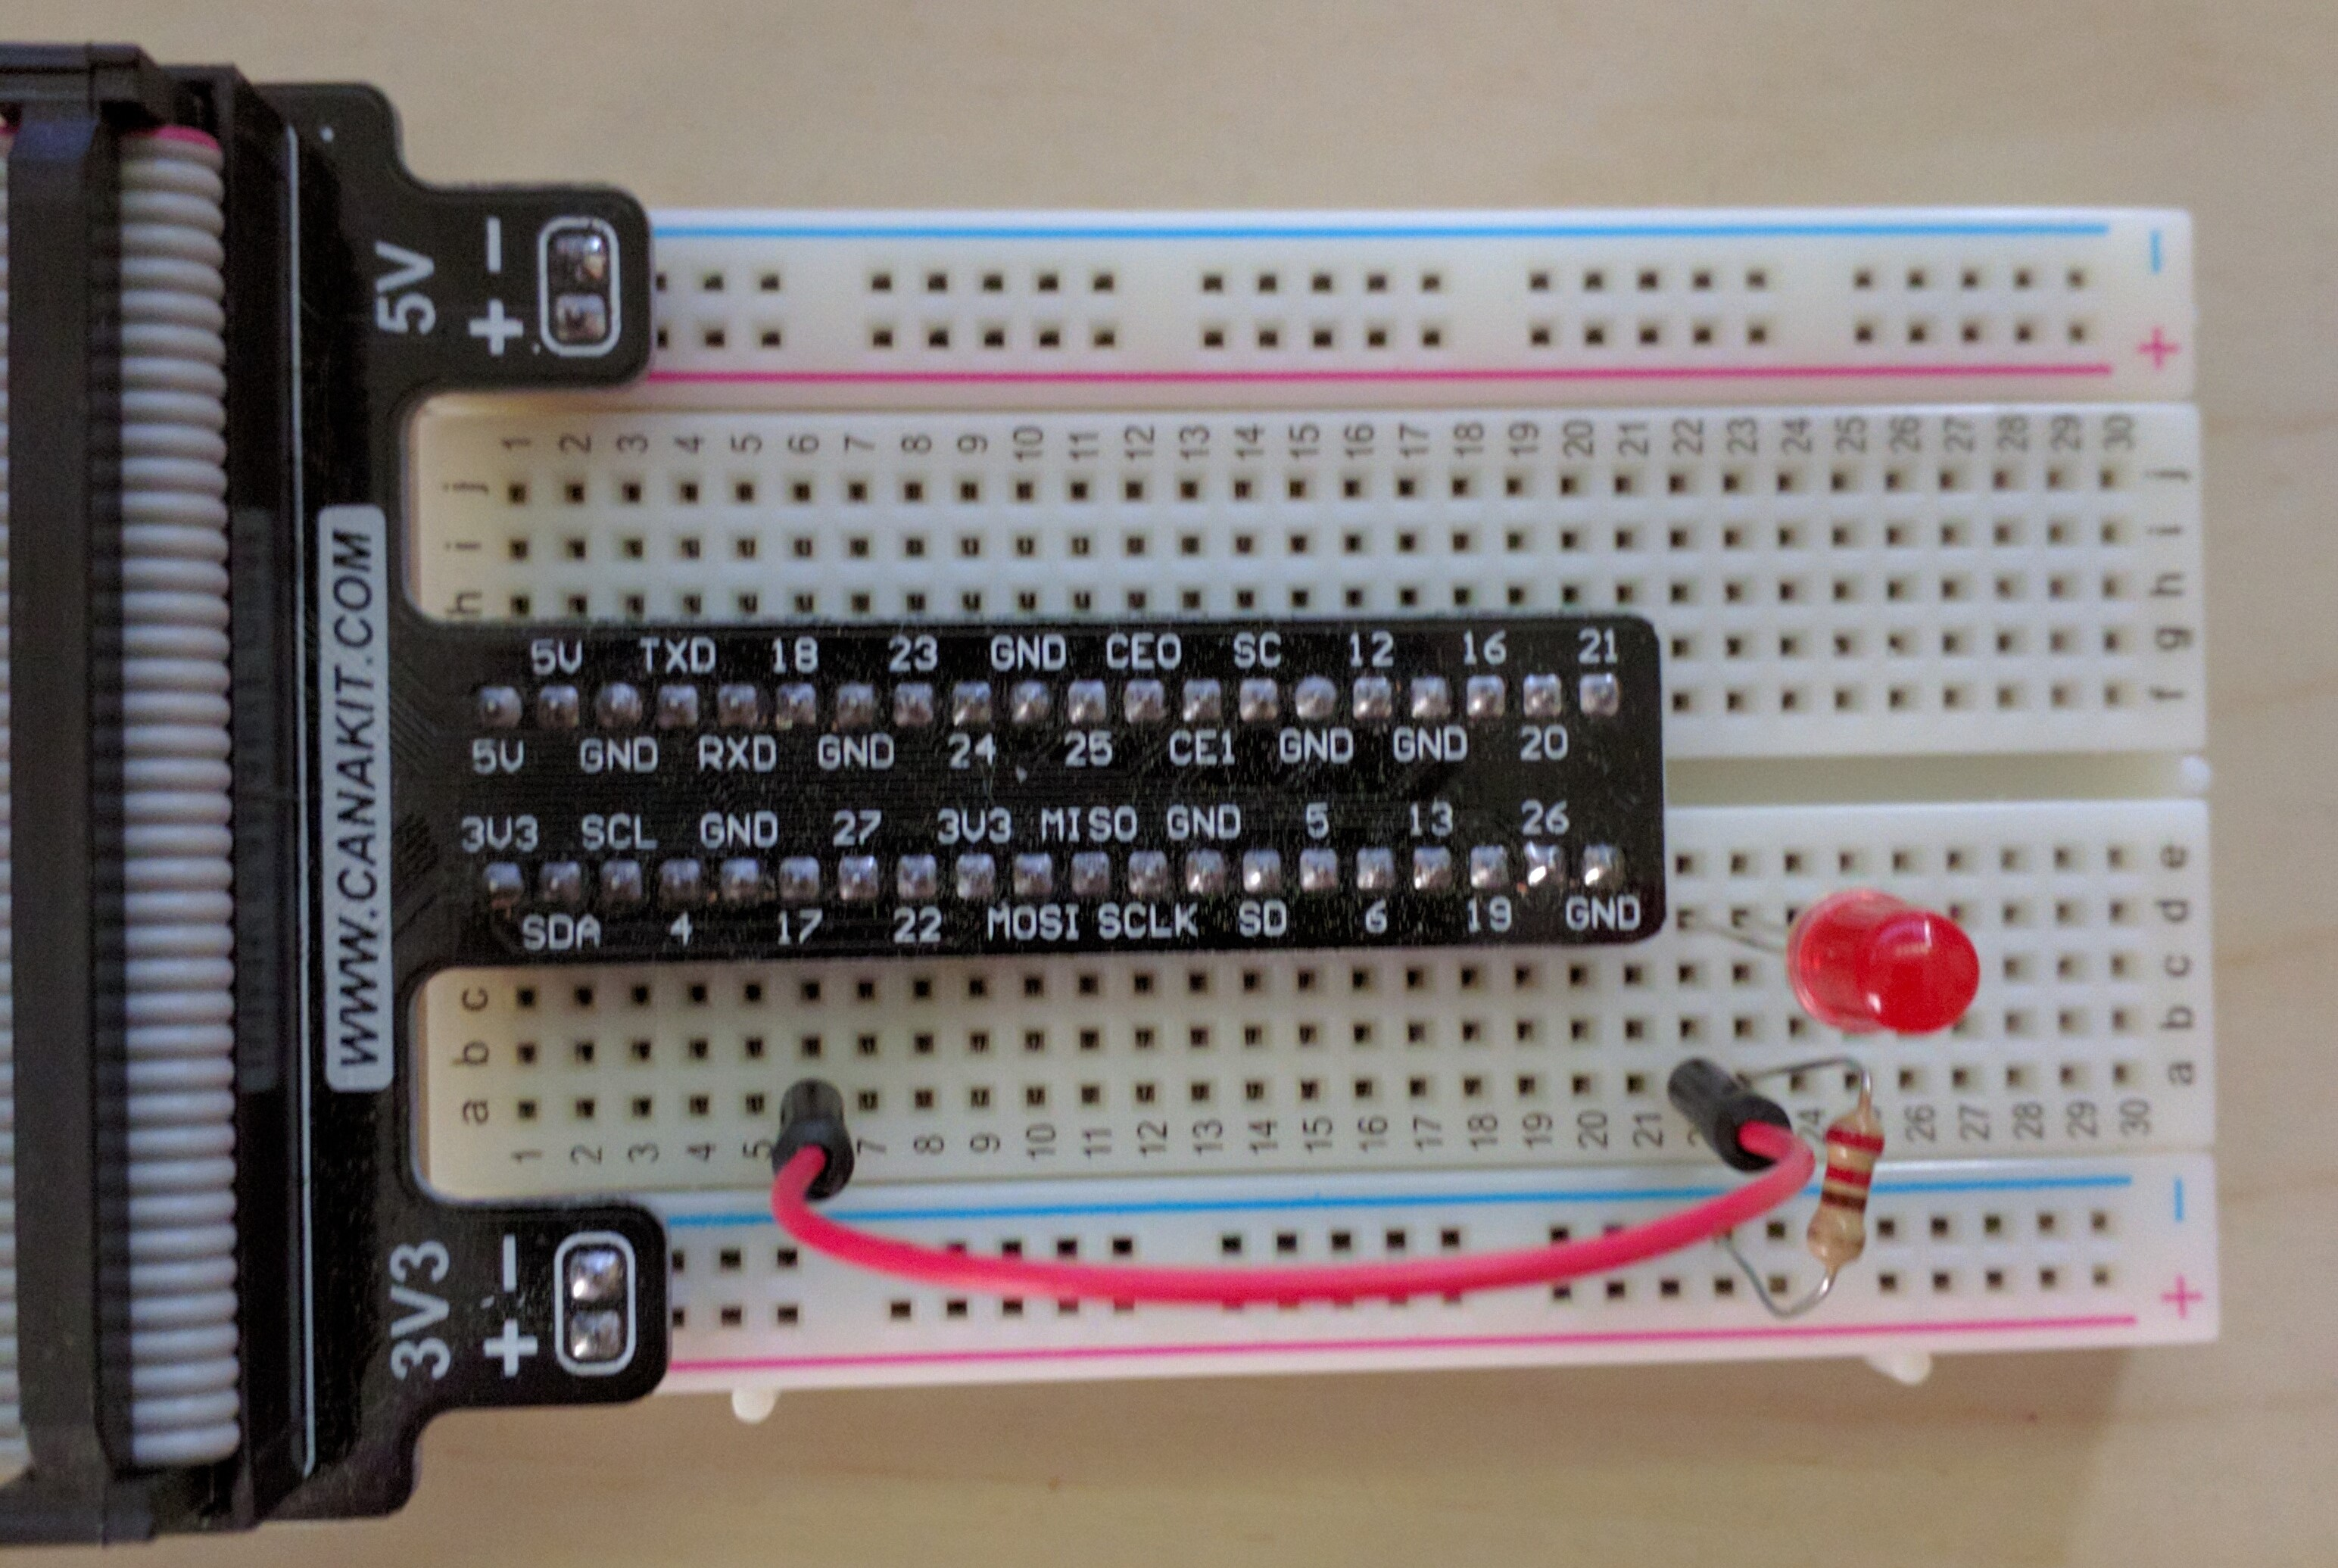
\includegraphics[height=2in]{pi_images/lab01images/PiLab01-1Light-photo.jpg}}
\afterfig

\underline{GPIO Assignments}

\begin{center}
	\begin{tabular}{c | c | c}
		\hline
		\textbf{Type} & \textbf{GPIO} & \textbf{Description} \\ \hline
		Led & 0 & Only LED for part 1 \\ 
		\hline	
	\end{tabular}
\end{center}

\vspace{10pt}

Start up your Pi and bring up the Eclipse environment. 	Remember to start the \textbf{PiLib Server}. Download and setup the PiLab01 project from the class website.

\underline{Run the Wiring Test}

Open the \textbf{\texttt{WiringTest}} program and run it. For information about wiring tests and common problems when testing your breadboard project please see the description on page \pageref{wiringTestDescription}.

\textbf{Program Implementation}

The project contains two additional source code files containing classes named \texttt{ControlOneLight} and \texttt{ControlTwoLights}. We will start by working on the \texttt{ControlOneLight} class, since we only have one light on our breadboard.

Open the source file for \texttt{ControlOneLight} and review the code. The class has a \texttt{main()} method containing all the code that controlls the light.

Our goal at this point is to walk through the code and understand what it is doing. First run the program and make sure the LED lights up. 

When the program runs it attempts to turn on the light for 2 seconds, turn it off for 2 seconds, make it blink for 4 seconds and finally turn it off as the program ends. If the LED isn't lighting up when you run the program, check your breadboard connections very carefully. If you can't find a problem, try a different LED, perhaps the one you are using is broken.

\textbf{Exploring the \texttt{ControlOneLight} Class}

This simple program uses most of the building blocks that we'll need for more advanced labs. Lets take the time to understand what the code is doing.

Here is the complete program:

\beforeverb
\begin{verbatim}
package edu.skidmore.cs106.pi.lab01;

import us.daveread.raspberrypi.gpio.lib.client.Led;
import us.daveread.raspberrypi.gpio.lib.client.Utility;
import us.daveread.raspberrypi.gpio.lib.client.Widget;

/**
 * Controls a single LED, turning it on, blinking and off.
 * @author readda
 */
public class ControlOneLight {
 /**
  * Creates an Led instance and uses different methods to control the LED.
  * @param args
  *          Command line arguments - not used
  */
 public static void main(String[] args) {
  // Reset old mappings
  Widget.gpioReset();

  // Declare an Led variable
  Led myLight;

  // Create an instance of the Led class
  myLight = new Led(0);

  // Turn the light on for 2 seconds
  myLight.turnOnSolid();
  Utility.pause(2000);

  // leave the light off for 2 seconds
  myLight.turnOff();
  Utility.pause(2000);

  // Make the light blink for 3 seconds
  myLight.turnOnBlink();
  Utility.pause(4000);

  // Turn off the light
  myLight.turnOff();

  System.out.println("Program ends");
 }
}
\end{verbatim}
\afterverb

The \texttt{package} and \texttt{import} statements are covered in other parts of the course. For our purposes note that the library classes that we are using are located in a separate package and need to be imported. You will generally just import these into each lab. One other class, Button, will also need to be imported when we starting using buttons.

As we've covered elsewhere, the program starts running by executing the code in the \texttt{main()} method.

The first statement we see is \texttt{Widget.gpioReset()}. Remember this assures that there aren't any old GPIO pin mappings left from some other program. It is a good practice to include this statement before setting up your widgets.

%The keywords \texttt{try} and \texttt{finally} are also covered separately in the class. When using the PiLib library for these labs simply follow this template approach to your main method:

%\begin{enumerate}
%	\item Start a \texttt{try} block
%	\item Write your code within the \texttt{try} block
%	\item End the \texttt{try} block
%	\item Start a \texttt{finally} block that contains one statement: %\texttt{GpioWidgetPool.close()}
%	\item End the {finally} block and the \texttt{main} method.
%\end{enumerate}

The next statement is a declaration of a variable named \texttt{myLight} of type \texttt{Led}. 

\beforeverb
\begin{verbatim}
Led myLight;
\end{verbatim}
\afterverb

The \texttt{Led} class represents a physical LED, providing the behaviors (methods) for turning it on and off.

Next we create an instance of the \texttt{Led} class and associate it with GPIO 0. We place that new instance in the variable, \texttt{myLight}, which we had declared above. Here is the statement that creates and assigns the instance:

\beforeverb
\begin{verbatim}
myLight = new Led(0);
\end{verbatim}
\afterverb

Note that the way we associate an instance of an Led (and we'll see this is true for any widget) with a GPIO number is to include that number within the parentheses as we create the instance. Put another way, the GPIO number is a parameter we pass to the Led class' constructor.

Now that we have an instance of an Led that is associated with a GPIO pin, we can use the class' methods to control the LED. The next statement turns on the Led connected to GPIO 0:

\beforeverb
\begin{verbatim}
myLight.turnOnSolid();
\end{verbatim}
\afterverb

We've seen this syntax in previous chapters but let's highlight what is happening. We are telling Java to use the Led instance stored in the variable \texttt{myLight} and to run the code in the method \texttt{turnOn()} on that instance. The \texttt{turnOn()} method is written to supply power to the instance's GPIO pin.

After this line of code executes the LED will be on. However, we need a way to make the program wait a couple of seconds so that the light stay on. Remember, by default the program just keeps executing its statements one after the other as fast as it can. 

In order to pause the program so that the light stays on for a couple of seconds we can use Java's ability to make a program "sleep" for a period of time. The \texttt{Utility} class contains a \texttt{pause()} method that we can use for this purpose. The method takes one parameter, the number of milliseconds to pause.

In the next statement we have our program pause for 2 seconds (2000 milliseconds).

\beforeverb
\begin{verbatim}
Utility.pause(2000);
\end{verbatim}
\afterverb


Our program will pause its execution for two seconds before moving onto the next statement. This means the light will stay on for those two seconds.

We next turn off the LED and have it remain off for two seconds. Here are the statements that do that:

\beforeverb
\begin{verbatim}
myLight.turnOff();
Utility.pause(2000);
\end{verbatim}
\afterverb

After those two seconds pass we turn on the light in blinking mode. We want it to blink for 4 seconds. Here are the statements for that operation:

\beforeverb
\begin{verbatim}
myLight.turnOnBlink();
Utility.pause(4000);
\end{verbatim}
\afterverb


Finally we turn the light off before exiting the program.

\beforeverb
\begin{verbatim}
myLight.turnOff();
\end{verbatim}
\afterverb

We end the program with a message on the console verifying that the program has ended.

\beforeverb
\begin{verbatim}
 System.out.println("Program ends");
 \end{verbatim}
\afterverb

\textbf{Note that if you don't remember to turn off the LEDs, they will remain on as long as the server program (PiLibServer) is running and the \texttt{Widget.gpioReset()} method hasn't been called.} If you want to assure that all LEDs are off when your program ends, simply include a call to \texttt{Widget.gpioReset()} at the end of your program.
	
\section{Lab 1 - Part 2}

\textbf{Learning Goals}

\begin{enumerate}
	\item Create a working circuit with 2 LEDs controlled by a Java program running on the Pi
	\item Creatively use the Led class methods that allow us to control our physical LEDs
	\item Reinforce the relationship between virtual objects (instances of a class) and their physical counterparts
\end{enumerate}

\textbf{Overview}

You will use your breadboard to connect two LEDs to two GPIO pins. With this setup you will write a Java program which controls the LEDs. 

\textbf{Breadboard Configuration}

\underline{Wiring Depiction}

\beforefig
\centerline{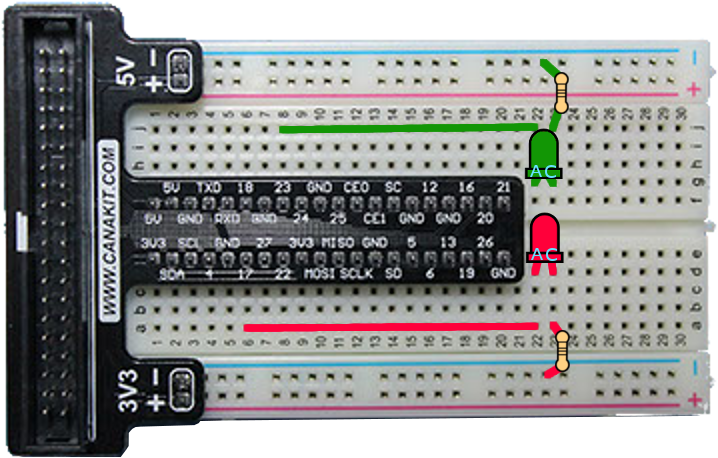
\includegraphics[height=2in]{pi_images/lab01images/PiLab01-2Light.png}}
\afterfig

\underline{Wiring Steps}

\textbf{Remember, your Pi must be disconnected from a power source while wiring the circuit.}

These steps assume your breadboard is setup as described in \textbf{Lab 1 - Part 1}. If it isn't , go through those wiring steps before returning to the ones below.

\begin{enumerate}
	\item Insert an LED anode (longer wire) into hole \textbf{g22}
	\item Insert the same LED's cathode into hole \textbf{g23}
	
	\item Insert a jumper from hole \textbf{j8} to hole \textbf{j22}

	\item Insert a resistor between hole \textbf{j23} and a \textbf{5V--} (negative) hole adjacent to row 23.
	
	\item If your ribbon cable is not connected to the Pi and the breakout board, connect it now (making sure your Pi is disconnected from any power source)
\end{enumerate}

\underline{Completed Breadboard Picture}

\beforefig
\centerline{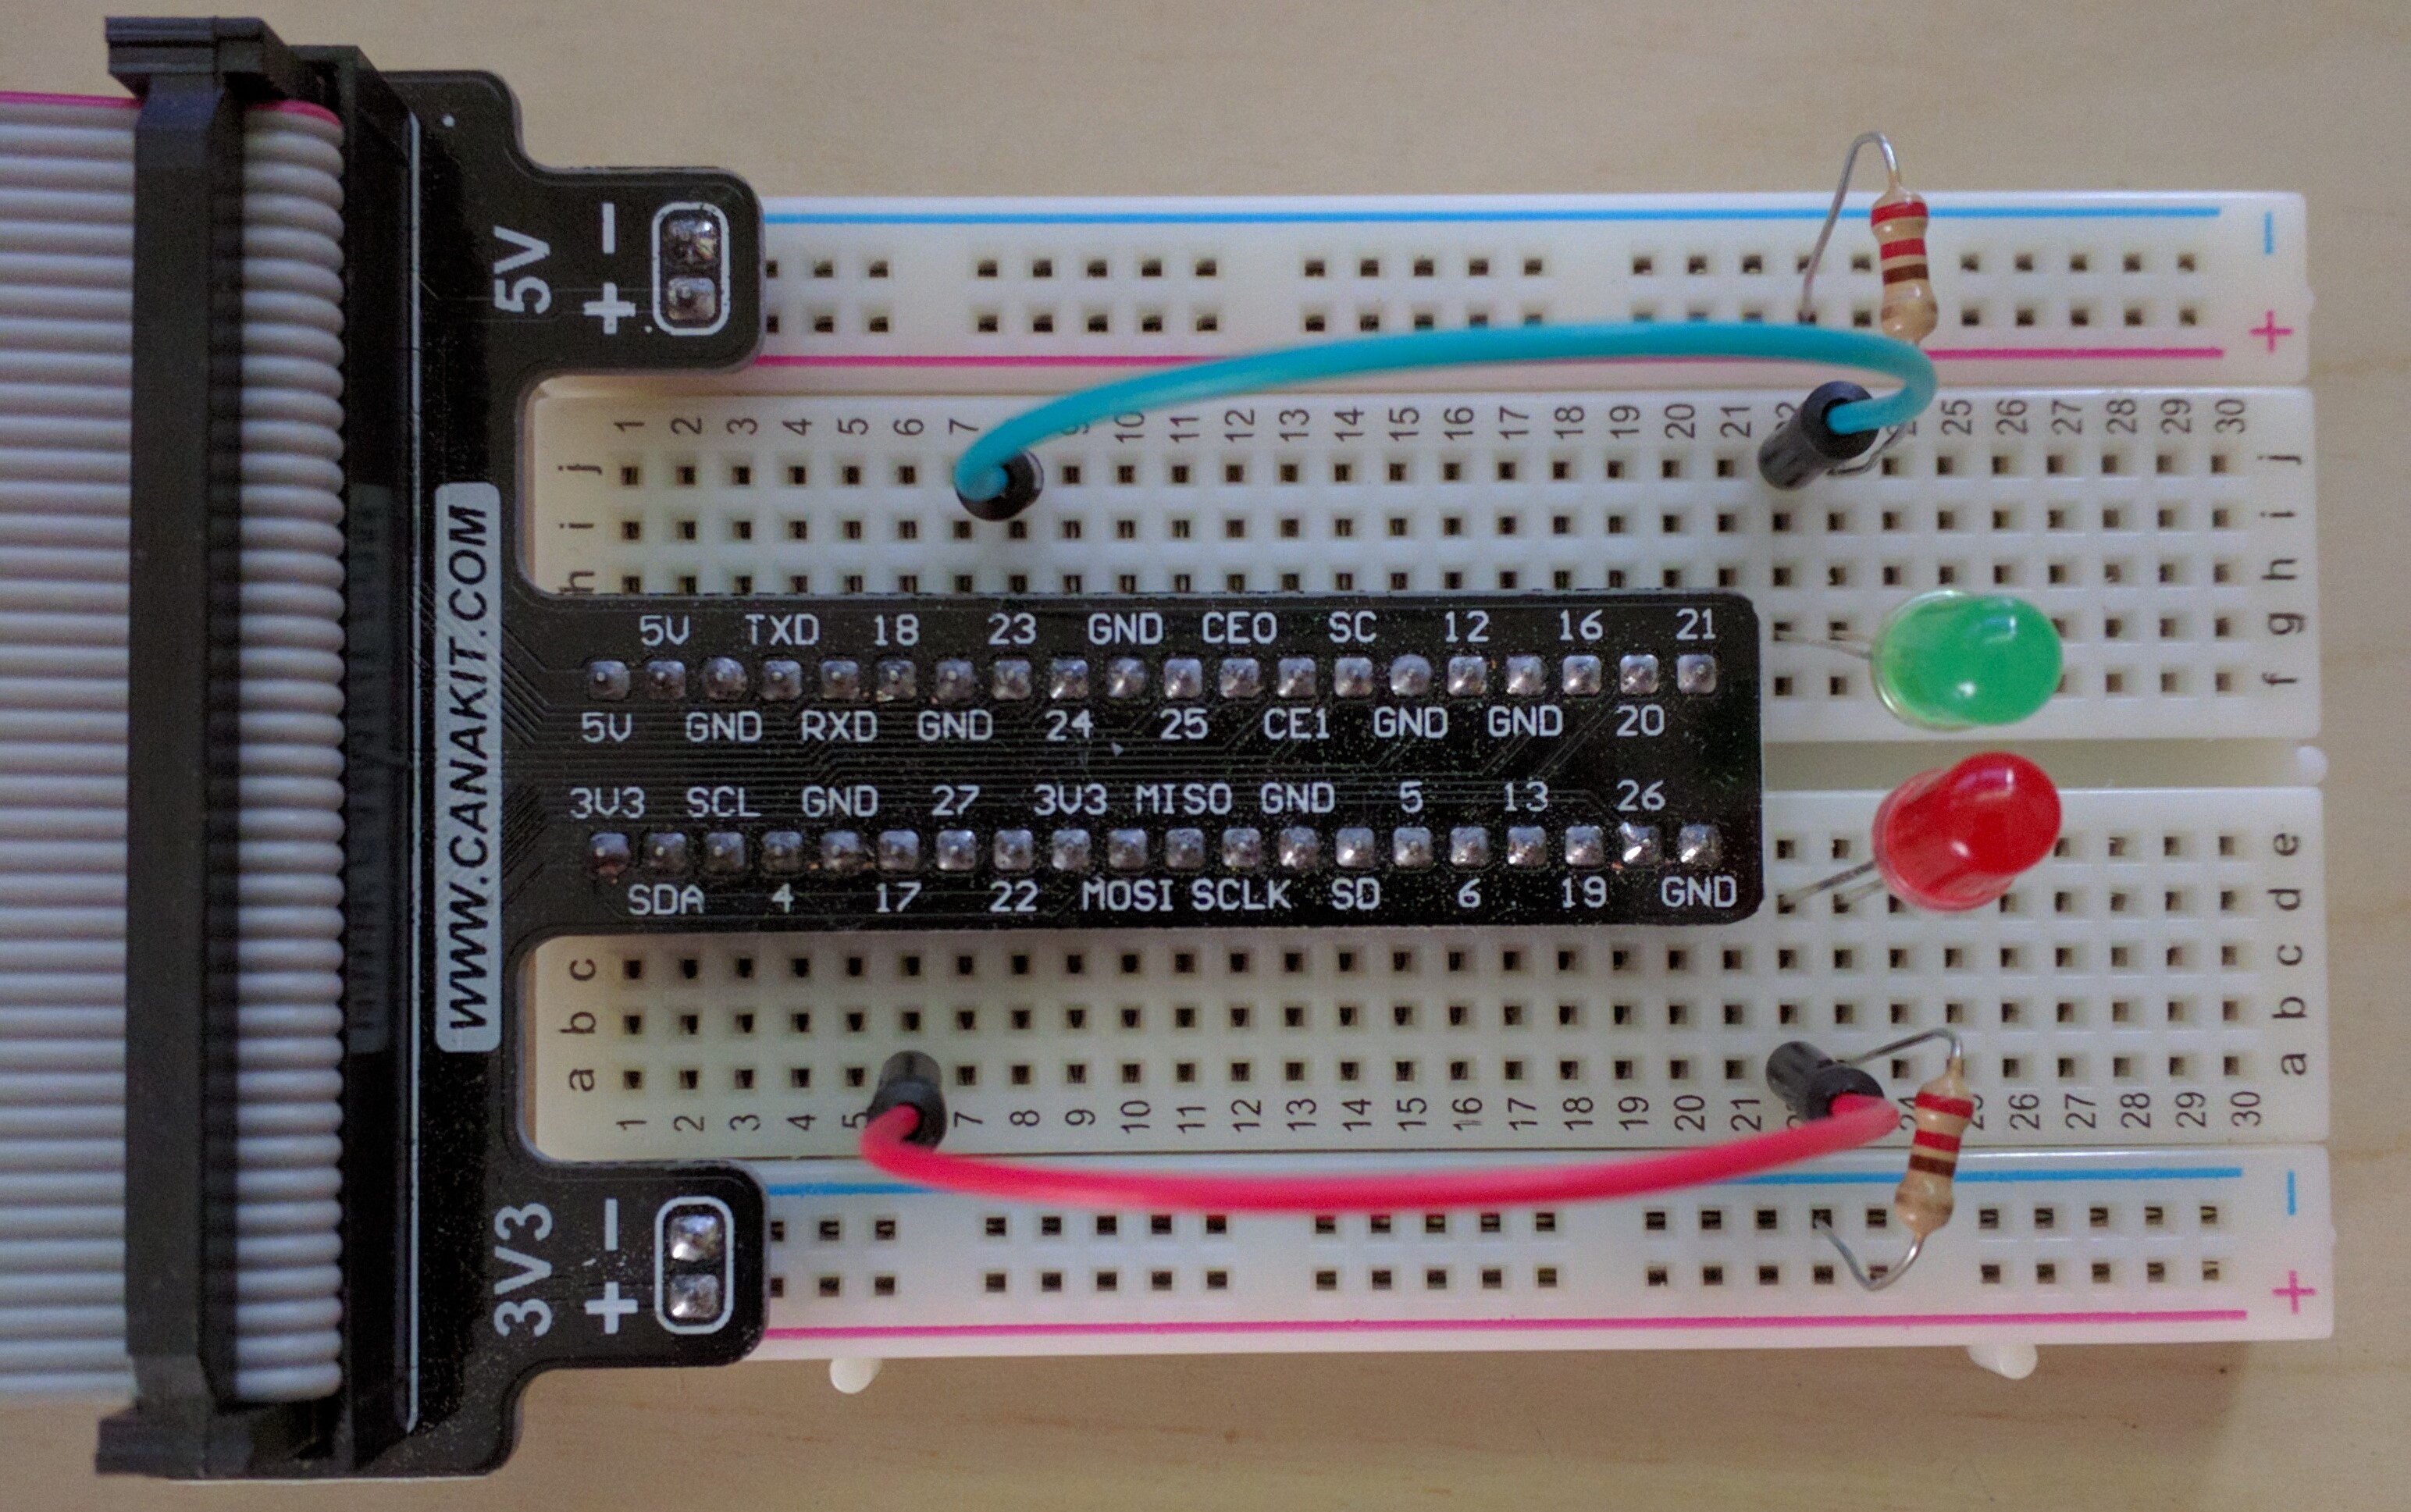
\includegraphics[height=2in]{pi_images/lab01images/PiLab01-2Light-photo.jpg}}
\afterfig

\underline{GPIO Assignments}

\begin{center}
	\begin{tabular}{c | c | c}
		\hline
		\textbf{Type} & \textbf{GPIO} & \textbf{Description} \\ \hline
		Led & 0 & First LED \\ 
		\hline
		Led & 4 & Second LED \\ 
		\hline	
	\end{tabular}
\end{center}

\vspace{10pt}

Start up your Pi and remember to start the \textbf{PiLib Server}.  Bring up the Eclipse environment. Return to the PiLab01 project (which you setup in part 1 of this lab).

\underline{Run the Wiring Test}

Open the \textbf{\texttt{WiringTest}} program and run it. For information about wiring tests and common problems when testing your breadboard project please see the description on page \pageref{wiringTestDescription}.

\textbf{Program Implementation}

Open the source file for \texttt{ControlTwoLights} and review the code. The class has a \texttt{main()} method with a \texttt{try} and \texttt{finally} blocks. 

The implementation code has not been supplied. Your job is to use the concepts you learned in part one of this lab and create a program that does the following:

\begin{enumerate}
	\item Declare two variables of type Led. Consider naming them \texttt{myFirstLight} and \texttt{mySecondLight} though you are free to name them something different if you prefer.
	\item Create an instance of an Led associated with GPIO 0 and assign it to your first Led variable. We will call this \textbf{LED 1}
	\item Create an instance of an Led associated with GPIO 4 and assign it to your second Led variable. We will call this \textbf{LED 2}
	\item Turn on LED 1 in blinking mode while turning on LED 2 so that it stays steadily lit.
	\item Pause your program for 3 seconds, allowing the LEDs to blink and illuminate
	\item Switch the LEDs so that your LED 1 stays on steadily and LED 2 blinks
	\item Pause your program for another 3 seconds
	\item Turn off LED 1 and set LED 2 to stay steadily lit
	\item Pause your program for half a second (500 milliseconds)
	\item Turn on LED 1 (steady) and turn off LED 2
	\item Pause your program for half a second (500 milliseconds)
	\item Repeat the prior 4 steps 2 more times. Our goal is to have the LEDs flashing back and forth when the program gets to this part of the code.
\end{enumerate}

Test your program and adjust your code until the steps are working. Go ahead and experiment by creating other outputs. 

For example can you figure out how to send the message "SOS" in Morse Code? S is three short signals and O is three long signals. We would write it out as:

\beforeverb
\begin{verbatim}
dot-dot-dot dash-dash-dash dot-dot-dot (...  ---  ...)
\end{verbatim}
\afterverb

Using the LEDs we could define "long" as 1 second and short as a quarter second (250 milliseconds). We could define the time between signals as a quarter second and the time between letters as 1 second. With those timings, the code you write to depict "SOS" will turn an LED on and off for the correct durations.

Your solution will end up being sets of \texttt{turnOn()} and \texttt{pause()} statements followed by \texttt{turnOff()} and \texttt{pause()} statements. A video of what this lab might end up looking like when run is located at: \url{https://youtu.be/2a2cu42BZHE}

\textbf{End of Lab}

This concludes lab 1. You've covered a lot of ground in terms of wiring up your breadboard and controlling devices from your Java program. We'll build more complex circuits and programs as we build on this foundation.

\textbf{Remember to submit your completed lab using the process defined by your instructor.}

{\centering
\beforefig
\centerline{
\includegraphics[height=1in]{pi_images/stop_sign_clip_art_16252.jpg}}
\afterfig
}

\newpage

\section{Lab 2 - Part 1}

\textbf{Learning Goals}

\begin{enumerate}
	\item Reinforce relationship between instances and physical LEDs
	\item Use user input to make decisions
\end{enumerate}

\textbf{Overview}

Create a circuit that has 4 LEDs. One of the 4 lights will be turned on based on keyboard input.

\textbf{Breadboard Configuration}

\underline{Wiring Depiction}

\beforefig
\centerline{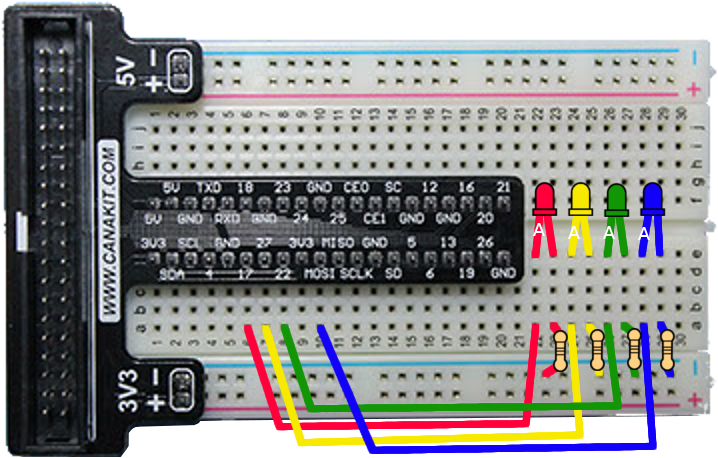
\includegraphics[height=2in]{pi_images/lab02images/PiLab02-4Light.png}}
\afterfig

\underline{Wiring Steps}

\textbf{Remember, your Pi must be disconnected from a power source while wiring the circuit.}

\begin{enumerate}
	\item Insert an LED anode into hole \textbf{e22}
	\item Insert the same LED's cathode into hole \textbf{e23}
	\item Insert an LED anode into hole \textbf{e24}
	\item Insert the same LED's cathode into hole \textbf{e25}
	\item Insert an LED anode into hole \textbf{e26}
	\item Insert the same LED's cathode into hole \textbf{e27}
	\item Insert an LED anode into hole \textbf{e28}
	\item Insert the same LED's cathode into hole \textbf{e29}

	\item Insert a jumper from hole \textbf{a6} to hole \textbf{a22}
	\item Insert a jumper from hole \textbf{a7} to hole \textbf{a24}
	\item Insert a jumper from hole \textbf{a8} to hole \textbf{a26}
	\item Insert a jumper from hole \textbf{a10} to hole \textbf{a28}

	\item Insert a resistor between hole \textbf{a23} and a \textbf{3V3--} hole adjacent to row 23
	\item Insert a resistor between hole \textbf{a25} and a \textbf{3V3--} hole adjacent to row 25
	\item Insert a resistor between hole \textbf{a27} and a \textbf{3V3--} hole adjacent to row 27
	\item Insert a resistor between hole \textbf{a29} and a \textbf{3V3--} hole adjacent to row 29
	
	\item If your ribbon cable is not connected do so now.
\end{enumerate}

\underline{Completed Breadboard Picture}

\beforefig
\centerline{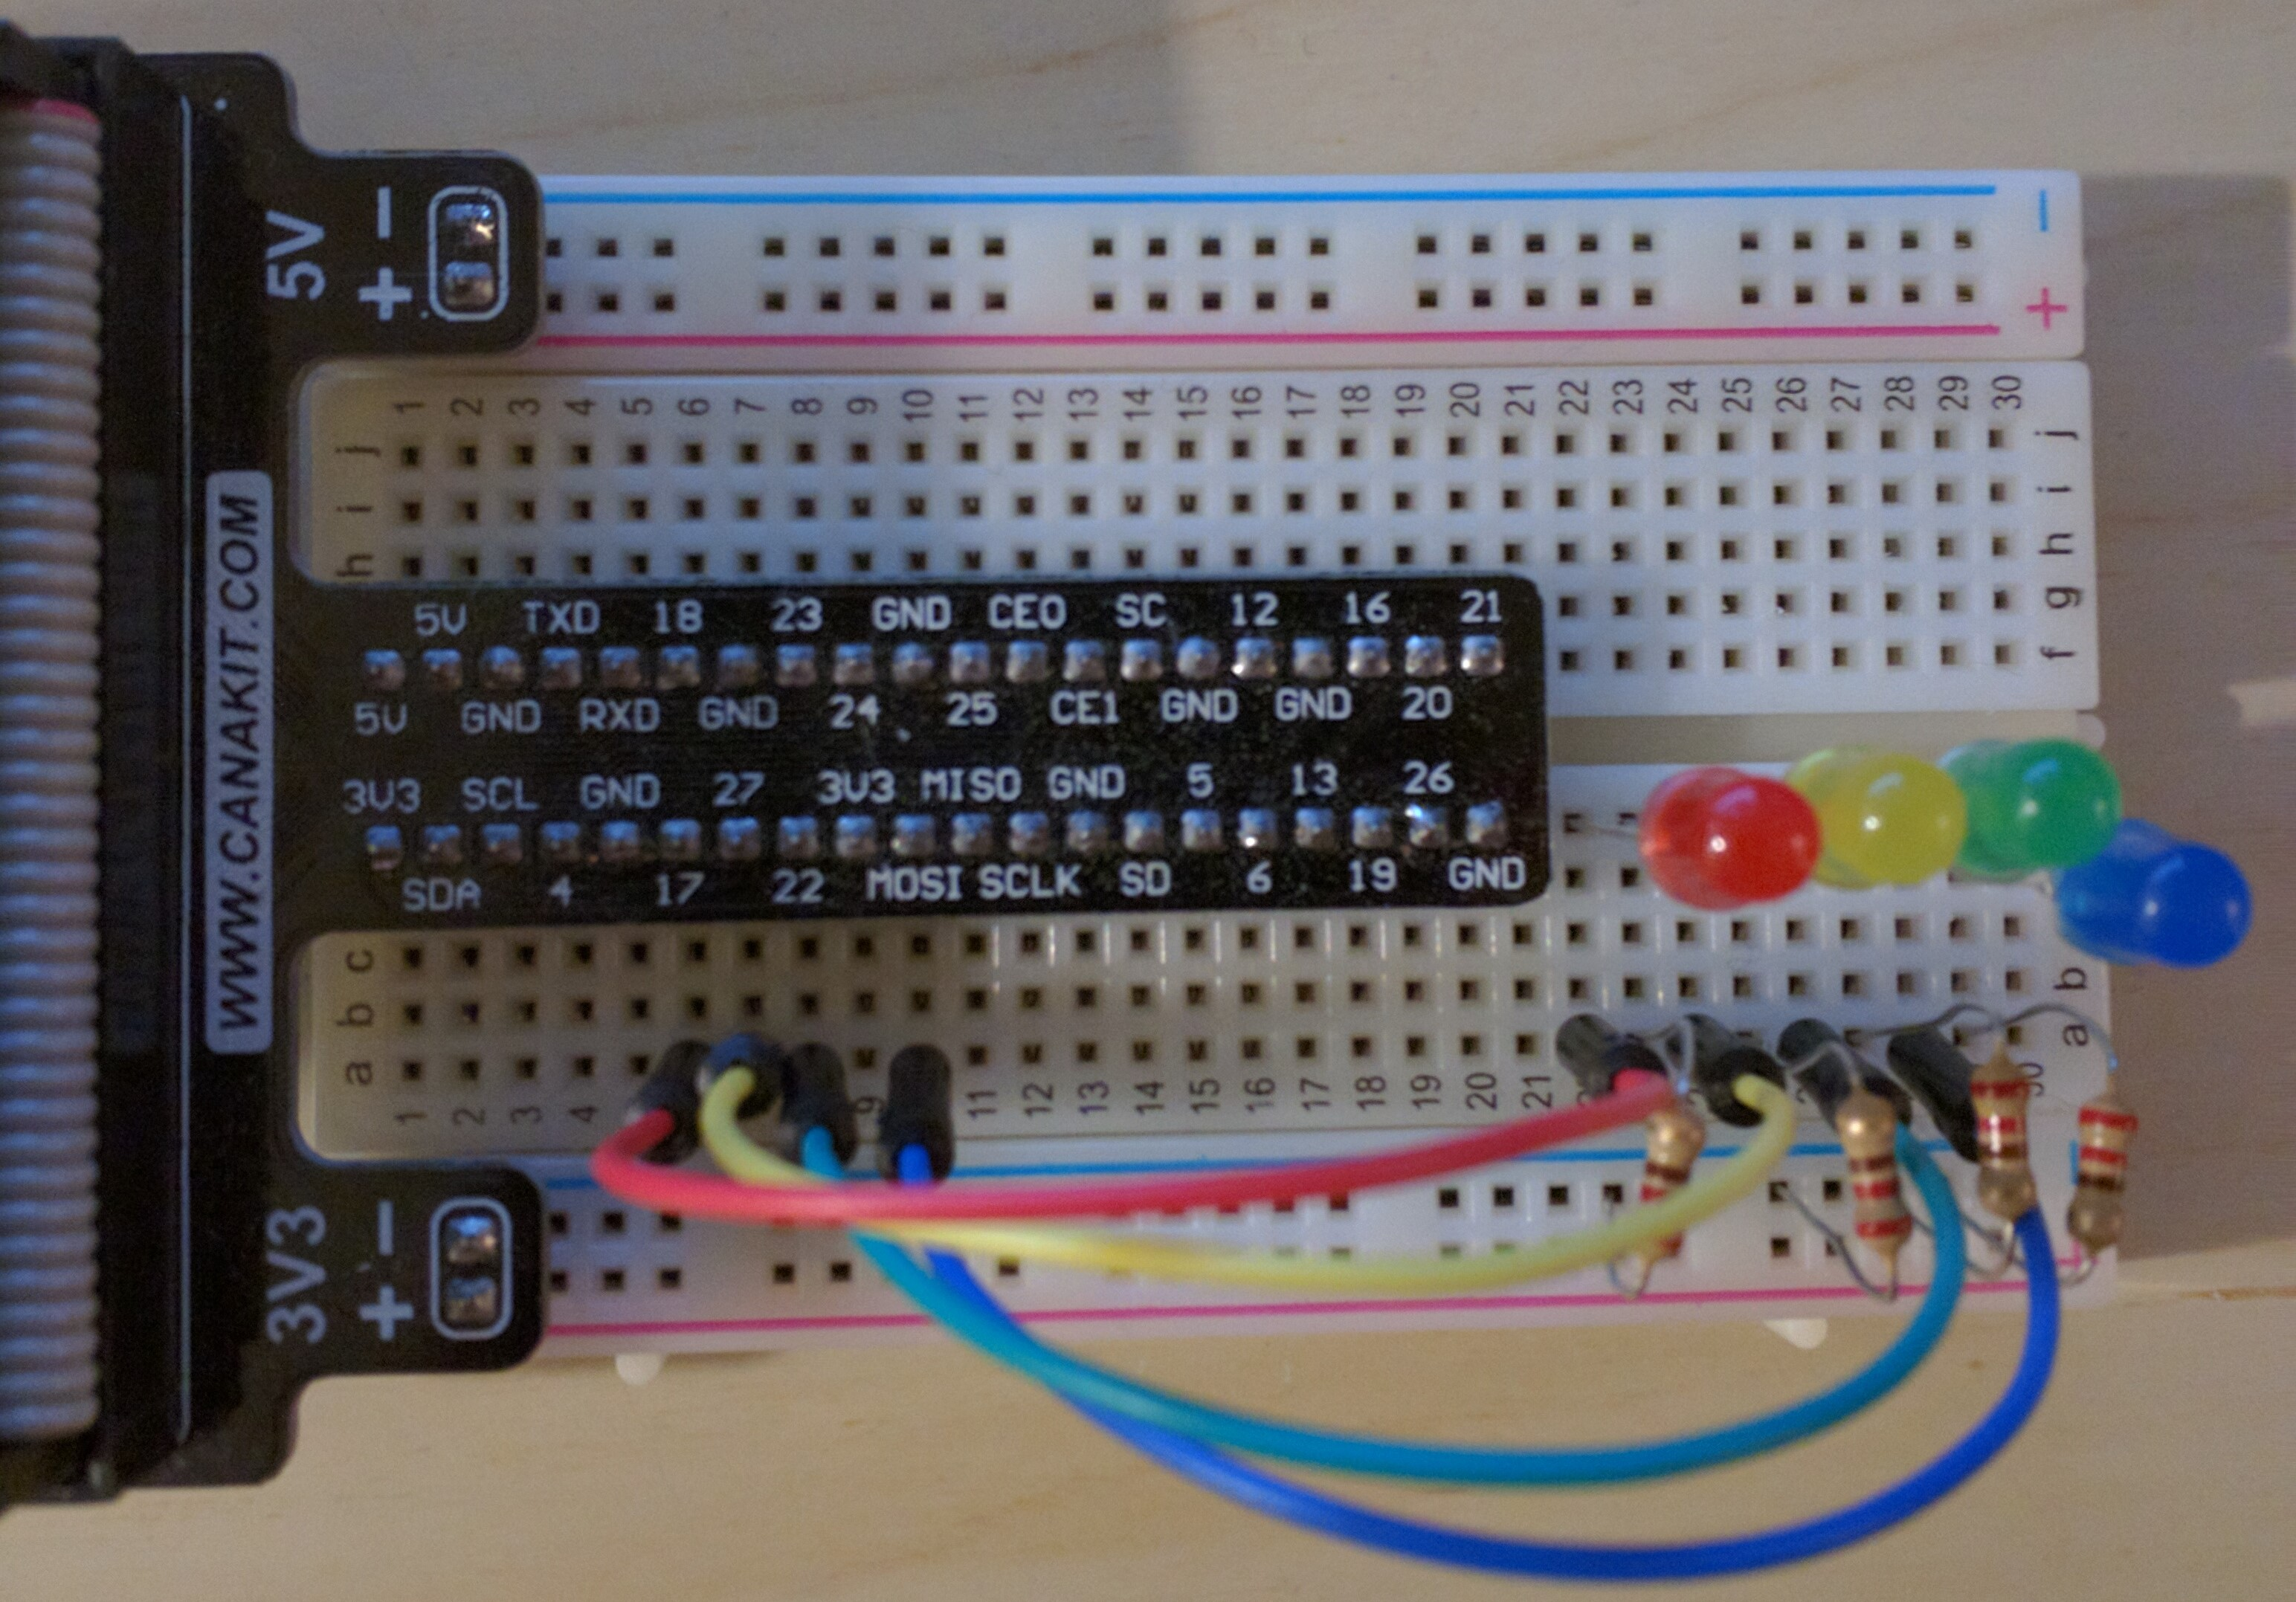
\includegraphics[height=2in]{pi_images/lab02images/PiLab02-4Light-photo.jpg}}
\afterfig

\underline{GPIO Assignments}

\begin{center}
	\begin{tabular}{c | c | c}
		\hline
		\textbf{Type} & \textbf{GPIO} & \textbf{Description} \\ \hline
		Led & 0 & First LED \\ 
		\hline
		Led & 2 & Second LED \\ 
		\hline
		Led & 3 & Third LED \\ 
		\hline
		Led & 12 & Fourth LED \\ 
		\hline	
	\end{tabular}
\end{center}

\vspace{10pt}

Start up your Pi and remember to start the \textbf{PiLib Server}. Bring up the Eclipse environment. Download and setup the PiLab02 project from the class website.

\underline{Run the Wiring Test}

Open the \textbf{\texttt{WiringTest}} program and run it. For information about wiring tests and common problems when testing your breadboard project please see the description on page \pageref{wiringTestDescription}.

\textbf{Program Implementation}

The project contains two source code files named \texttt{ControlWhichLight} and \texttt{ControlWhichAndHowLight}. We'll start by creating the code for the \texttt{ControlWhichLight} class, so open that file. The class has an empty \texttt{main()} method. You will write the code for this method.

When the program runs the user will be prompted to use the keyboard to enter a value telling the program which light to turn on. The program will then turn on the corresponding LED. The program will then wait for the user to press the \texttt{Enter} key, at which point the program ends.

Use the \texttt{Utility.readKeyboardLine()} method to get the String the user entered.

Each LED should light up when a certain String value is entered by the user. For example if the user types ``1" the first LED should light up. If the user types ``2" the second LED should light up. ``3" corresponds to the 3rd LED and ``4" corresponds to the 4th LED.

As an alternative to using \texttt{Utility.pause()} to force the LED to stay on for a few seconds at the end of the program, you can instead print a message telling the user to press \textbf{Enter} to exit the program and then call \texttt{Utility.readKeyboardLine()}.

\section{Lab 2 - Part 2}

\textbf{Overview}

Allow the user to choose which LED to turn on and if the light should blink or be solid.

\textbf{Breadboard Configuration}

Same as for part 1.

\textbf{Program Implementation}

In this part of the lab you will modify the code you wrote in part 1. You will use the \texttt{ControlWhichAndHowLight} class for this part of the lab. Start by copying your code from the \texttt{main()} method in \texttt{ControlWhichLight} to the \texttt{main()} method in \texttt{ControlWhichAndHowLight}. 

\textit{Now change the \texttt{ControlWhichAndHowLight} program as follows:}

When the program runs the user should be prompted to choose the LED they want to light up (as you did in part 1). The user will then be prompted to choose if they want the light to blink or be solid, perhaps using the letters ``b" and ``s" as the choices. The chosen light should then light up. So that the light stays on long enough to see, either use a \texttt{Utility.pause()} or \texttt{Utility.readKeyboardLine()} to keep the program from immediately ending, and thereby turning off the LED.

For example, if the user wants the first light to be solid the user would enter ``1" to the first prompt and ``s" to the second prompt. If the user wants to fourth light to blink they would enter ``4" to the first prompt and ``b" to the second.

\textbf{End of Lab}

This concludes lab 2. You controlled many LEDs with one program and learned how to make decisions based on user input. In the next lab you'll see how to use buttons instead of keyboard inputs in your programs.

\textbf{Remember to submit your completed lab using the process defined by your instructor.}

{\centering
	\beforefig
	\centerline{
\includegraphics[height=1in]{pi_images/stop_sign_clip_art_16252.jpg}}
	\afterfig
}

\newpage

\section{Lab 3 - Part 1}

\textbf{Learning Goals}

\begin{enumerate}
	\item Use buttons as a source of user input
	\item See how loops can be used with buttons to control a program
\end{enumerate}

\textbf{Overview}

In part one you will explore a program that uses buttons to stop and end a program. In part two you will allow the user to use a button to turn a light on and off and another button to decide when to end the program.

\textbf{Breadboard Configuration}

\underline{Wiring Depiction}

\beforefig
\centerline{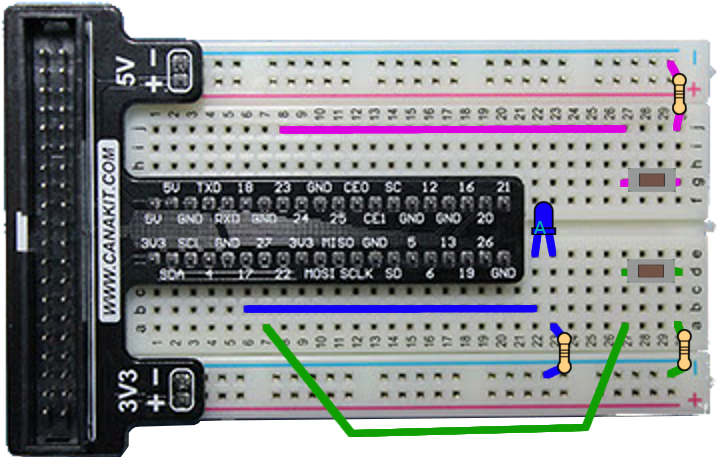
\includegraphics[height=2in]{pi_images/lab03images/PiLab03-ButtonLight.png}}
\afterfig

\underline{Wiring Steps}

\textbf{Remember, your Pi must be disconnected from a power source while wiring the circuit.}

\begin{enumerate}
	\item Insert a button into holes \textbf{d27} and \textbf{d30}
	\item Insert a button into holes \textbf{g27} and \textbf{g30}

    
    \item Insert the anode of an LED into hole \textbf{e22} the cathode into hole \textbf{e23}
            
    \item Insert a jumper from hole \textbf{b6} to hole \textbf{b22}
    \item Insert a jumper from hole \textbf{a7} to hole \textbf{a27}
    \item Insert a jumper from hole \textbf{j8} to hole \textbf{j27}
    
    \item Insert a resistor from hole \textbf{a23} to a \textbf{3V3--} hole adjacent to row 23    
    \item Insert a resistor from hole \textbf{a30} to a \textbf{3V3--} hole adjacent to row 30
    \item Insert a resistor from hole \textbf{j30} to a \textbf{5V--} hole adjacent to row 30
        
    \item If your ribbon cable is not connected do so now.
\end{enumerate}

\underline{Completed Breadboard Picture}

\beforefig
\centerline{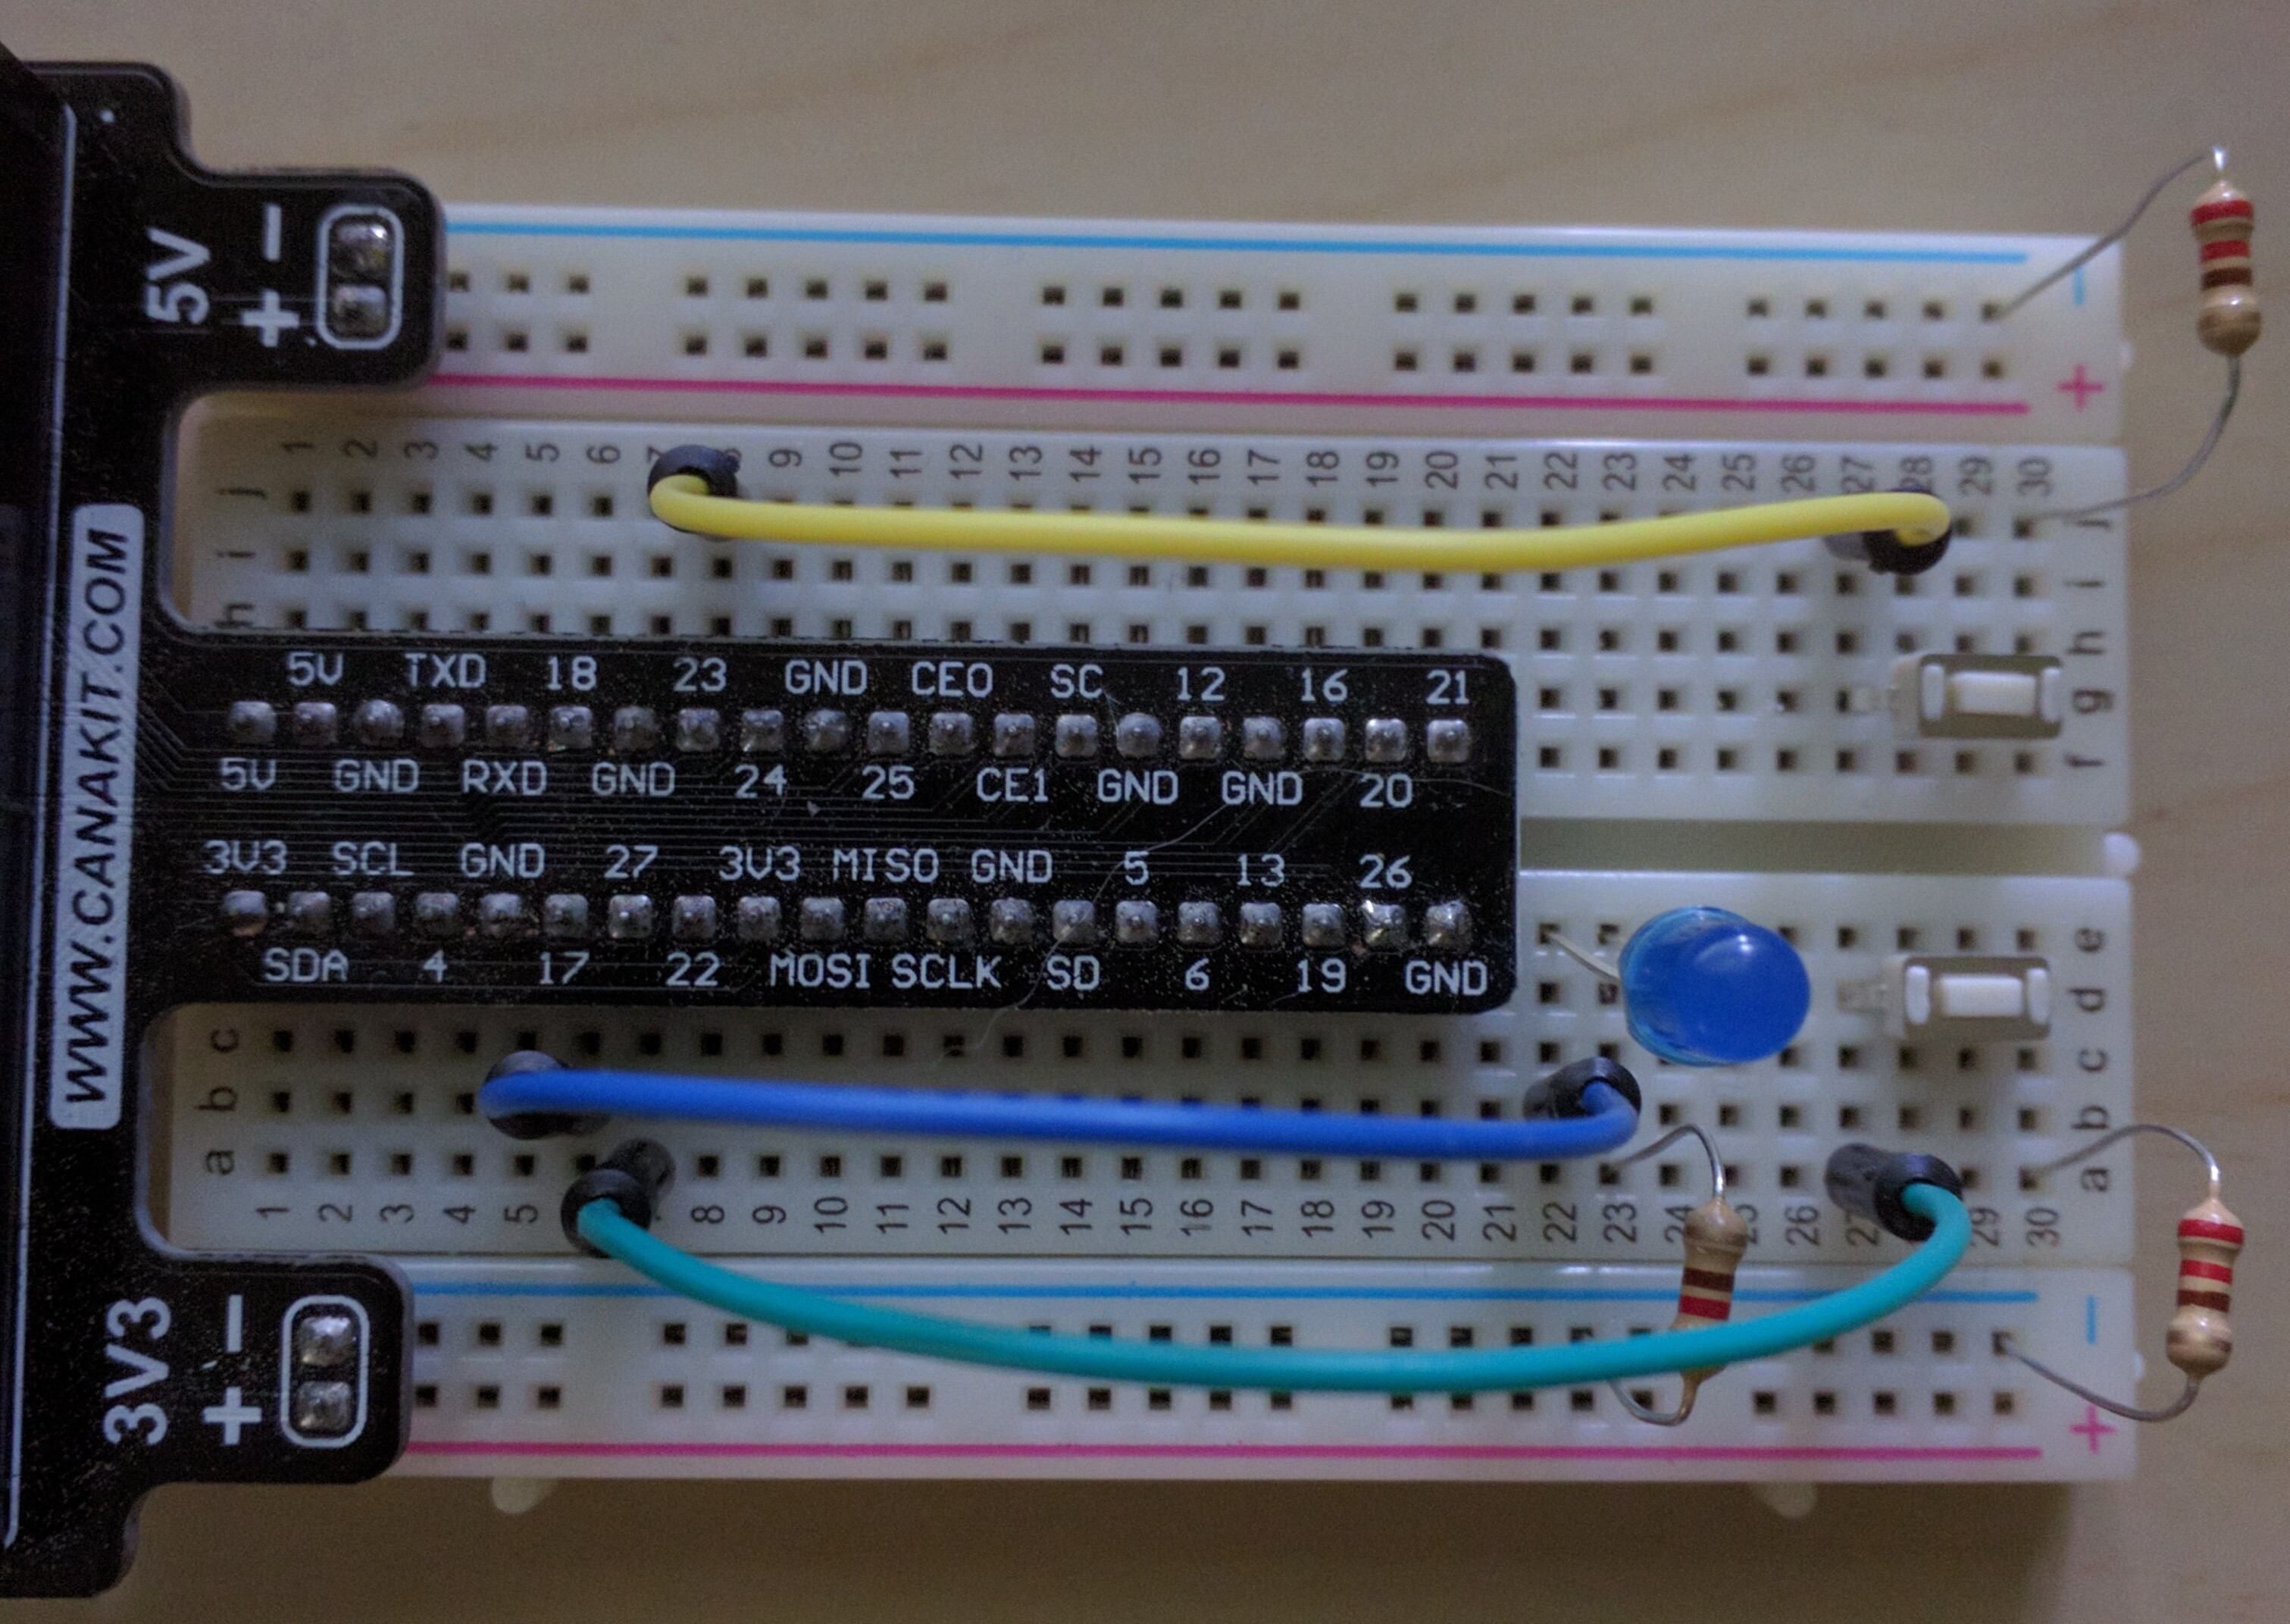
\includegraphics[height=2in]{pi_images/lab03images/PiLab03-ButtonLightPhoto.jpg}}
\afterfig

\underline{GPIO Assignments}

\begin{center}
	\begin{tabular}{c | c | c}
		\hline
		\textbf{Type} & \textbf{GPIO} & \textbf{Description} \\ \hline
		Led & 0 & Only LED used \\ 
		\hline
		Button & 2 & Left-hand button (start output) \\ 
		\hline
		Button & 4 & Right-hand button (end program) \\ 
		\hline	
	\end{tabular}
\end{center}

\vspace{10pt}

Start up your Pi and remember to start the \textbf{PiLib Server}. Bring up the Eclipse environment. Download and setup the PiLab03 project from the class website.

\underline{Run the Wiring Test}

Open the \textbf{\texttt{WiringTest}} program and run it. For information about wiring tests and common problems when testing your breadboard project please see the description on page \pageref{wiringTestDescription}.

\textbf{Program Implementation}

The project contains two source code files for two classes named \texttt{ControlProgramWithButton} and \texttt{ControlLightWithButton}. We will start by working on the \texttt{ControlProgramWithButton} class. We'll use this to learn how to use the Button class.

Open the source file for \texttt{ControlProgramWithButton} and review the code. The class has a \texttt{main()} method containing all the code that uses the buttons.

Our goal at this point is to walk through the code and understand what it is doing. First, let's run the program and make sure the buttons are working.

When the program runs it waits (up to 10 seconds) for the user to press the left-hand (GPIO 2) button. Once pressed, the program starts outputting random numbers. The program will keep running until the user presses the right-hand (GPIO 4) button. 

\textit{If the program isn't detecting the button being pressed}, check your breadboard connections very carefully. If you can't find a problem, make sure the button is seated properly on the breadboard. Sometimes the button's pins don't make contact within the breadboard.

\textbf{Exploring the \texttt{ControlProgramWithButton} Class}

This simple program uses the two buttons in two different ways. Lets take the time to understand what the code is doing.

Here is the complete program:

\beforeverb
\begin{verbatim}
package edu.skidmore.cs106.pi.lab03;

import java.util.Random;

import us.daveread.raspberrypi.gpio.lib.client.Button;
import us.daveread.raspberrypi.gpio.lib.client.Utility;
import us.daveread.raspberrypi.gpio.lib.client.Widget;

/**
 * Uses two buttons to control the program's behavior.
 * @author readda
 */
public class ControlProgramWithButton {
  /**
   * Use one button to start outputting random numbers. Use the other button
   * to end the program.
   * @param args
   *          Command line arguments - not used
   */
 public static void main(String[] args) {
  // Reset old mappings
  Widget.gpioReset();

  // Declare a Button variable
  Button startProgram;

  // Declare another Button variable
  Button endProgram;

  // Declare a Random variable
  Random randomNumberGenerator;

  // Create an instance of the Button class tied to GPIO 2
  startProgram = new Button(2);

  // Create another instance of the Button class tied to GPIO 4
  endProgram = new Button(4);

  // Create and instance of the Random class
  randomNumberGenerator = new Random();

  // Output a message to the console telling the user to press the
  // button
  System.out.println("Press the GPIO 2 button to start showing random numbers");
  System.out.println("Otherwise, the program will start outputting number in 10 seconds");

  // Wait for the button to be pressed (max wait will be 10000
  // milliseconds which is 10 seconds)
   startProgram.waitForPress(10000);

  // Keep looping until the GPIO 4 button is pressed. Each time
  // through the loop will output a random number and the message telling
  // the user how to stop the program. The program will pause for one
  // half-second between iterations.
  while (endProgram.getPressCount() == 0) {
   System.out.println("Your random number is: " + randomNumberGenerator.nextInt());
   System.out.println("Press the GPIO 4 button to end the program\n");
   Utility.pause(500);
  }

  System.out.println("The program has ended.");
 }
}
\end{verbatim}
\afterverb

Note that the Button class is being imported similar to how we were importing the Led class in previous labs.

Lets explore the code inside the \texttt{main()} method.

The first statement we see is \texttt{Widget.gpioReset()}. Remember this assures that there aren't any old GPIO pin mappings left from some other program. It is a good practice to include this statement before setting up your widgets.

The next two statements declare variables named \texttt{startProgram} and \texttt{endProgram} of type \texttt{Button}. 

\beforeverb
\begin{verbatim}
Button startProgram;
Button endProgram;
\end{verbatim}
\afterverb

The \texttt{Button} class represents a physical button, providing the behaviors (methods) for detecting when a button is pressed and how many times it has been pressed.

The next statement declares a variable named \texttt{randomNumberGenerator} of type \texttt{Random}. We've used the \texttt{Random} class in other labs. It gives us an easy way to create random numbers so that our program doesn't keep outputting the same value over and over. 

\beforeverb
\begin{verbatim}
Random randomNumberGenerator;
\end{verbatim}
\afterverb

Next we create two instances of the \texttt{Button} class and associate them with GPIO 2 and GPIO 4. We place the new instances in the variables, \texttt{startProgram} and \texttt{endProgram}, which we had declared above. Here are the statements that create and assign the instances:

\beforeverb
\begin{verbatim}
startProgram = new Button(2);
endProgram = new Button(4);
\end{verbatim}
\afterverb

Note that the way we associate an instance of a Button (as we saw with the Led class) with a GPIO number is to include that number within the parentheses as we create the instance. Put another way, the GPIO number is a parameter we pass to the Button class' constructor.

We then create an instance of \texttt{Random} and assign it to the \texttt{randomNumberGenerator} variable.

\beforeverb
\begin{verbatim}
randomNumberGenerator = new Random();
\end{verbatim}
\afterverb

Now that we have our instances setup we are ready to use the buttons to control the program. 

We want the program to wait until the user presses the left-hand button (connected to GPIO 2 and named \texttt{startProgram}) before it starts outputting random numbers. The \texttt{Button} class defines the method \texttt{waitForPress()} that pauses the program until one of two things happen:

\begin{enumerate}
	\item The user presses the button; or
	\item The timeout for waiting for the button to be pressed is reached
\end{enumerate}

The \textbf{timeout} value is supplied to the \texttt{waitForPress()} method as a number indicating the maximum number of milliseconds the program should wait for the button to be pressed. The timeout feature is simply included so that if something is wrong with the breadboard's wiring, the program won't get permanently stuck waiting for the button press.\footnote{The fancy term for this type of method, one that stops the program until another event occurs (like pressing a button), is a \textbf{blocking call} or \texttt{synchronous call}. It is called this because the program is blocked from running until the event occurs. If you're wondering if there are such things as \texttt{non-blocking calls} the answer is "yes." They allow the program to keep running while they do their work and are also known as \textbf{asynchronous calls}.}

Before having the program wait for the button press, we need to let the user know that we are waiting on an action so that he or she knows what to do. We output a message to that effect. Here is the code that informs the user about pressing the button and then waits for the button to be pressed.


\beforeverb
\begin{verbatim}
System.out
  .println("Press the GPIO 2 button to start showing random numbers");
System.out
  .println("Otherwise, the program will start outputting number in 10 seconds");
startProgram.waitForPress(10000);
\end{verbatim}
\afterverb

As with using the Led instance, we've seen this syntax in previous chapters but let's again review what is happening. We are telling Java to use the Button instance stored in the variable \texttt{startProgram} and to run the code in the method \texttt{waitForPress()} on that instance. The \texttt{waitForPress()} method is written to pause the program until the user presses the button (or the timeout value is reached).

Once the left-hand button has been pressed we want the program to continuously output random numbers until the user presses the right-hand button (connected to GPIO 4 and named \texttt{endProgram}). We use a \texttt{while} loop to keep running the same code repeatedly (outputting the random numbers) until the lower button is pressed. 

We use a different approach to detecting the button press in this case. We don't want the program to stop running while we wait for the button to be pressed. Instead we just want to check whether it hs been pressed, and if not, continue running. The \texttt{Button} class defines another method, \texttt{getPressCount()} which allows us to detect if it has been pressed without waiting for it to be pressed. When you call \texttt{getPressCount()} it returns the number of times the button has been pressed. If it has not been pressed the value will be zero (0).

Our loop can then simply check the count of times that the \texttt{endProgram} button has been pressed. As long as that number is zero, the loop should keep running. Once it isn't zero, the loop must exit. Here is the loop control code that enforces that rule:

\beforeverb
\begin{verbatim}
while (endProgram.getPressCount() == 0) {
\end{verbatim}
\afterverb

The work inside the loop is to output a random number, remind the user how to end the program and then delay for a half-second so that the user has some opportunity to read the information scrolling by on the screen. Here is the remainder of the loop:

\beforeverb
\begin{verbatim}
 System.out.println("Your random number is: "
   + randomNumberGenerator.nextInt());
 System.out
   .println("Press the GPIO 4 button to end the program\n");
 Utility.pause(500);
}
\end{verbatim}
\afterverb

As verification so that the user knows that the button press to end the program was detected a message is printed indicating that the program is ended.

\beforeverb
\begin{verbatim}
System.out.println("The program has ended.");
\end{verbatim}
\afterverb

This ends the \texttt{main} method, which means the program will end as well.

\section{Lab 3 - Part 2}

\textbf{Learning Goals}

\begin{enumerate}
	\item Use a button to control an LED and another button to cause the program to end
	\item Reinforce the relationship between virtual objects (instances of a class) and their physical counterparts
\end{enumerate}

\textbf{Overview}

Using the existing breadboard setup you will write a Java program which controls an LED via a button.

\textbf{Breadboard Configuration}

Same as for part 1.

\textbf{Program Implementation}

Start up your Pi and bring up the Eclipse environment. Return to the PiLab03 project (which you setup in part 1 of this lab).

Open the source file for \texttt{ControlLightWithButton}. The class has a \texttt{main()} method with no code. You will write the code for this method.

When the program runs, the user will press the left-hand button to change the state of the light (turn the light on or off). The program will run until the user presses the right-hand button.

\textbf{\underline{Extra Challenge}} \newline
For an additional challenge, have the light cycle between off, blinking, and on as the user presses the left-hand button.

\textbf{End of Lab}

This concludes lab 3. You used multiple buttons to take in user input and learned how to use \texttt{while} loops along with checking whether a button has been pressed. In the next lab you'll use what you have learned so far to build a traffic light.

\textbf{Remember to submit your completed lab using the process defined by your instructor.}

{\centering
	\beforefig
	\centerline{
\includegraphics[height=1in]{pi_images/stop_sign_clip_art_16252.jpg}}
	\afterfig
}


\newpage

\section{Lab 4 - Part 1}

\textbf{Learning Goals}

\begin{enumerate}
	\item Work with multiple Led and Button instances
	\item Manage the state of different LEDs as button inputs are received
\end{enumerate}

\textbf{Overview}

Create a circuit that has 3 LEDs and 2 buttons. The 3 LEDs are intended to mimic a standard three-light traffic signal. Use the upper button to cycle the light from green to yellow to red and back to green. The lower button is used to end the program.

\textbf{Breadboard Configuration}

\underline{Wiring Depiction}

\beforefig
\centerline{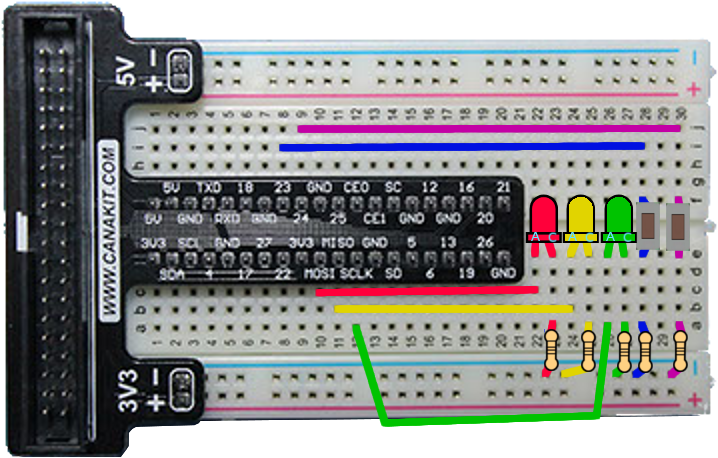
\includegraphics[height=2in]{pi_images/lab04images/PiLab04-StopLight.png}}
\afterfig

\underline{Wiring Steps}

\textbf{Remember, your Pi must be disconnected from a power source while wiring the circuit.}

\begin{enumerate}
	\item Insert a button in row 28 (e28 and f28)
	\item Insert a button in row 30 (e30 and f30)
	
	\item Insert the anode of an LED (red) into hole \textbf{e22} the cathode into hole \textbf{e23}
	\item Insert the anode of an LED (yellow) into hole \textbf{e24} the cathode into hole \textbf{e25}
	\item Insert the anode of an LED (green) into hole \textbf{e26} the cathode into hole \textbf{e27}
	
	\item Insert a jumper from hole \textbf{c10} to hole \textbf{c22}
	\item Insert a jumper from hole \textbf{b11} to hole \textbf{b24}
	\item Insert a jumper from hole \textbf{a12} to hole \textbf{a26}
	
	\item Insert a jumper from hole \textbf{i8} to hole \textbf{i28}
	\item Insert a jumper from hole \textbf{j9} to hole \textbf{j30}
	
	\item Insert a resistor from hole \textbf{a23} to a \textbf{3V3--} hole adjacent to row 23
	\item Insert a resistor from hole \textbf{a25} to a \textbf{3V3--} hole adjacent to row 25
	\item Insert a resistor from hole \textbf{a27} to a \textbf{3V3--} hole adjacent to row 27	
	\item Insert a resistor from hole \textbf{a28} to a \textbf{3V3--} hole adjacent to row 28
	\item Insert a resistor from hole \textbf{a30} to a \textbf{3V3--} hole adjacent to row 30
	
	\item If your ribbon cable is not connected do so now.
\end{enumerate}

\underline{Completed Breadboard Picture}

\beforefig
\centerline{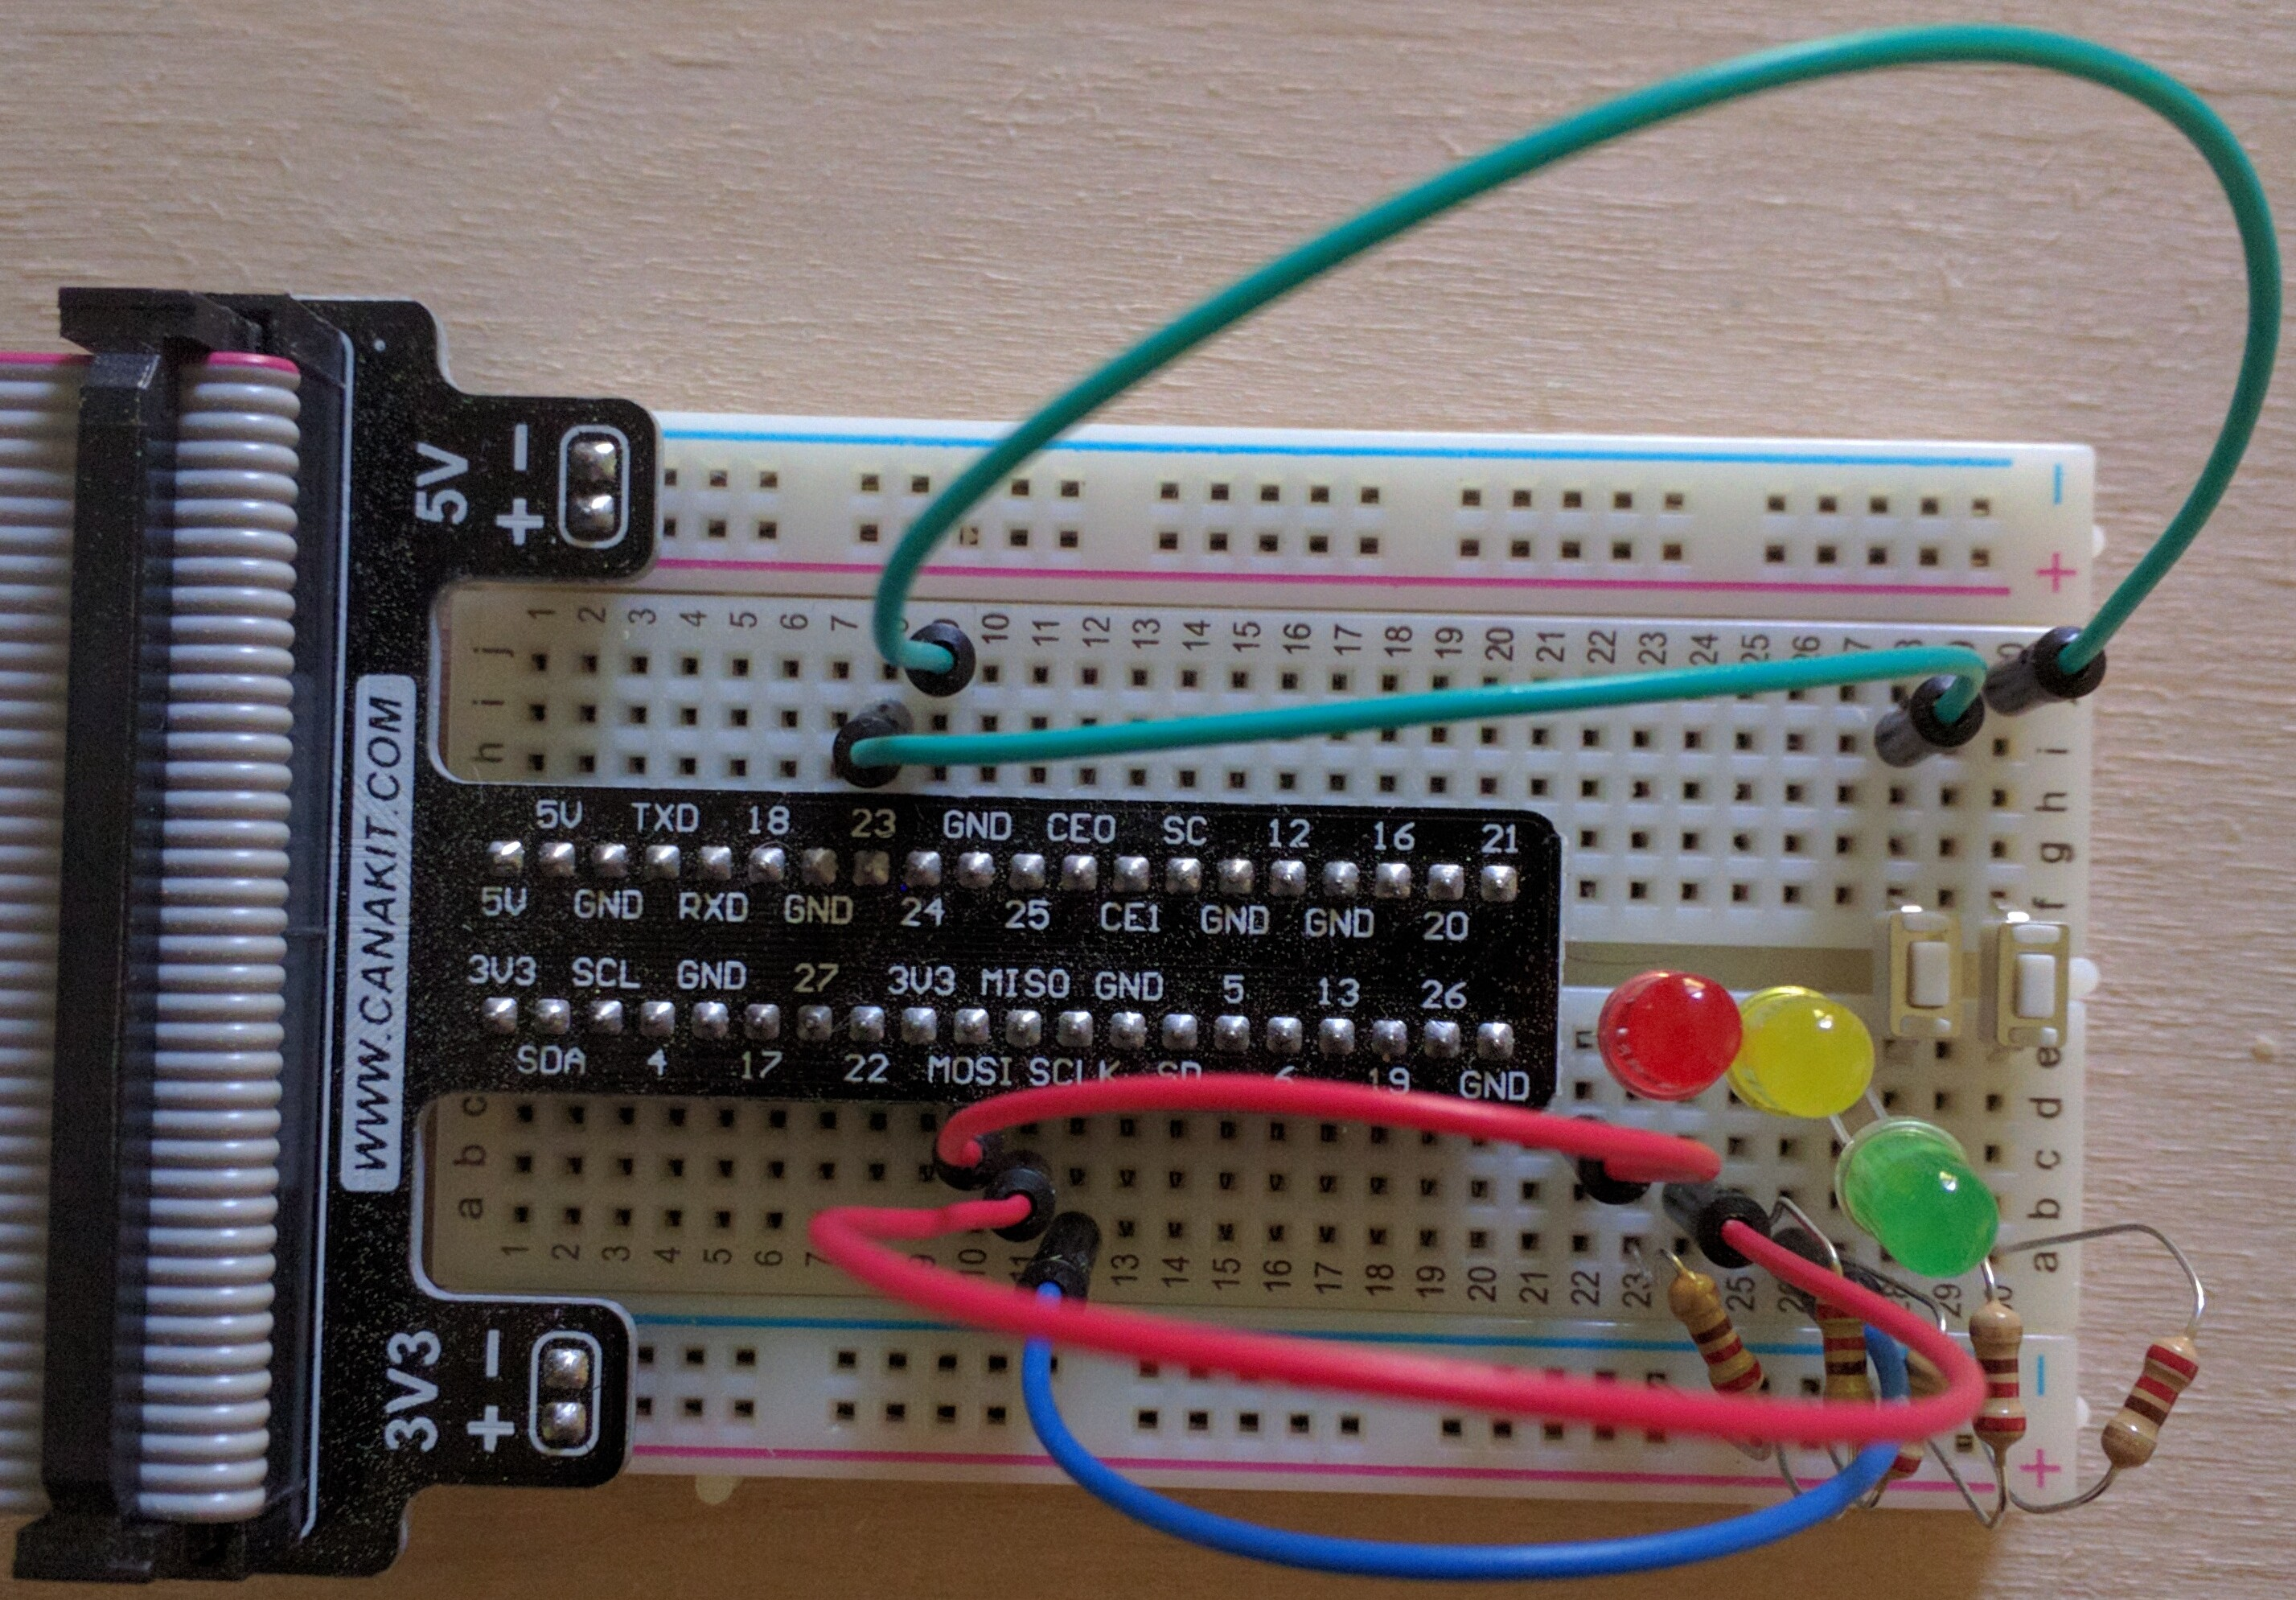
\includegraphics[height=2in]{pi_images/lab04images/PiLab04-StopLightPhoto.jpg}}
\afterfig

\underline{GPIO Assignments}

\begin{center}
	\begin{tabular}{c | c | c}
		\hline
		\textbf{Type} & \textbf{GPIO} & \textbf{Description} \\ \hline
		Led & 12 & First LED (red) \\ 
		\hline
		Led & 13 & Second LED (yellow) \\ 
		\hline
		Led & 14 & Third LED (green) \\ 
		\hline
		Button & 4 & First button (cycle color) \\ 
		\hline
		Button & 5 & Second button (end program) \\ 
		\hline	
	\end{tabular}
\end{center}

\vspace{10pt}

Start up your Pi and remember to start the \textbf{PiLib Server}. Bring up the Eclipse environment. Download and setup the PiLab04 project from the class website.

\underline{Run the Wiring Test}

Open the \textbf{\texttt{WiringTest}} program and run it. For information about wiring tests and common problems when testing your breadboard project please see the description on page \pageref{wiringTestDescription}.

\newpage

\textbf{Program Implementation}

The project contains two source code files named \texttt{ControlTrafficLightManual} and \texttt{ControlTrafficLightAutomatic}. The first part of the lab involves writing the code that manually controls the lights. Open the \texttt{ControlTrafficLightManual} class to begin working. This class has an empty \texttt{main()} method. You will write the code for this method.

\textit{Your program is to work as follows:}

When the program runs the green light should be turned on by default. Each time the user presses the upper button the light should cycle to the next light in the sequence (green to yellow to red and back to green, like a standard traffic light). If the user presses the lower button the program ends.

There is one challenge you should plan for. You'll need to turn off the previous LED when you are turning on the next one.\footnote{Generally, it would be confusing to a driver if two of the lights were on simultaneously} 

A video of what this lab might end up looking like when run is located at: \url{https://youtu.be/B0zkpa2Jbo0}

\section{Lab 4 - Part 2}

\textbf{Overview}

Automate the traffic light and use the upper button to switch between two automated modes. 

\textbf{Breadboard Configuration}

Same as for part 1.

\textbf{Program Implementation}

For this part of the lab open the \texttt{ControlTrafficLightAutomatic} class. The class has an empty \texttt{main()} method. You will write the code for this method.

For this program you will create a traffic light that is automated (e.g. the user doesn't press a button to make it change colors). Instead, the upper button causes the automated traffic light to switch between two modes of operation. The two modes are:

\begin{enumerate}
	\item The traffic light cycles through green to yellow to red and back to green, repeatedly. The student is free to choose the timings for each color. Note that for traditional traffic lights, yellow is lit for a relatively short amount of time compared to green or red.
	\item The traffic light simply flashes the red light (yellow and green are never turned on)
\end{enumerate}

Every time the user presses the upper button, the automated mode of operation switches between the two listed above. Similar to part one, you'll need to be sure to account for turning off lights as other lights are turned on. Pressing the lower button causes the program to end.

A video of what this lab might end up looking like when run is located at: \url{https://youtu.be/H1ZX3ZFs3i8}

\textbf{End of Lab}

This concludes lab 4. You cycled through a set of LEDs based on button input as well as automated timings.

\textbf{Remember to submit your completed lab using the process defined by your instructor.}

{\centering
	\beforefig
	\centerline{
\includegraphics[height=1in]{pi_images/stop_sign_clip_art_16252.jpg}}
	\afterfig
}

\newpage

\section{Lab 5 - Part 1}

\textbf{Learning Goals}

\begin{enumerate}
	\item Work with multiple LEDs and Buttons
	\item Manage the states of multiple LEDs as values are generated
\end{enumerate}

\textbf{Overview}

Create a circuit that has 7 LEDs and 2 buttons. The 7 LEDs will be used to display the 6 different values of a die. One button will be used to roll the die (and clear the roll value). The other will be used to end the program.

\textbf{Breadboard Configuration}

\underline{Wiring Depiction}

\beforefig
\centerline{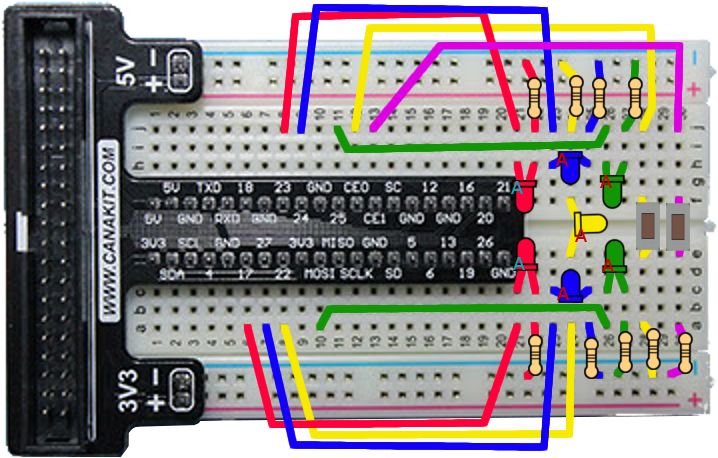
\includegraphics[height=2in]{pi_images/lab05images/PiLab05-DieLight.png}}
\afterfig

\underline{Wiring Steps}

\textbf{Remember, your Pi must be disconnected from a power source while wiring the circuit.}

\begin{enumerate}
	\item Insert a button in row 28 (e28 and f28)
	\item Insert a button in row 30 (e30 and f30)
	
	\item Insert the anode of an LED (red) into hole \textbf{c21} the cathode into hole \textbf{c22}
	\item Insert the anode of an LED (blue) into hole \textbf{c23} the cathode into hole \textbf{c25}
	\item Insert the anode of an LED (green) into hole \textbf{c26} the cathode into hole \textbf{c27}
	
	\item Insert the anode of an LED (yellow) into hole \textbf{e24} the cathode into hole \textbf{f24}
	
	\item Insert the anode of an LED (red) into hole \textbf{h21} the cathode into hole \textbf{h22}
	\item Insert the anode of an LED (blue) into hole \textbf{h23} the cathode into hole \textbf{h25}
	\item Insert the anode of an LED (green) into hole \textbf{h26} the cathode into hole \textbf{h27}

	\item Insert a jumper from hole \textbf{a6} to hole \textbf{a21}
	\item Insert a jumper from hole \textbf{a7} to hole \textbf{a23}
	\item Insert a jumper from hole \textbf{a8} to hole \textbf{a24}
		
	\item Insert a jumper from hole \textbf{a10} to hole \textbf{a26}

	\item Insert a jumper from hole \textbf{j8} to hole \textbf{j21}
	\item Insert a jumper from hole \textbf{j9} to hole \textbf{j23}
	\item Insert a jumper from hole \textbf{j11} to hole \textbf{j26}
	
	\item Insert a jumper from hole \textbf{j12} to hole \textbf{j28}
	\item Insert a jumper from hole \textbf{j13} to hole \textbf{j30}
	
	\item Insert a resistor from hole \textbf{a22} to a \textbf{3V3--} hole adjacent to row 22
	\item Insert a resistor from hole \textbf{a25} to a \textbf{3V3--} hole adjacent to row 25
	\item Insert a resistor from hole \textbf{a27} to a \textbf{3V3--} hole adjacent to row 27	
	\item Insert a resistor from hole \textbf{a28} to a \textbf{3V3--} hole adjacent to row 28
	\item Insert a resistor from hole \textbf{a30} to a \textbf{3V3--} hole adjacent to row 30
	\item Insert a resistor from hole \textbf{j22} to a \textbf{5V--} hole adjacent to row 22
	\item Insert a resistor from hole \textbf{j24} to a \textbf{5V--} hole adjacent to row 24	
	\item Insert a resistor from hole \textbf{j25} to a \textbf{5V--} hole adjacent to row 25
	\item Insert a resistor from hole \textbf{j27} to a \textbf{5V--} hole adjacent to row 27
	
	\item If your ribbon cable is not connected do so now.
\end{enumerate}

\underline{Completed Breadboard Picture}

\beforefig
\centerline{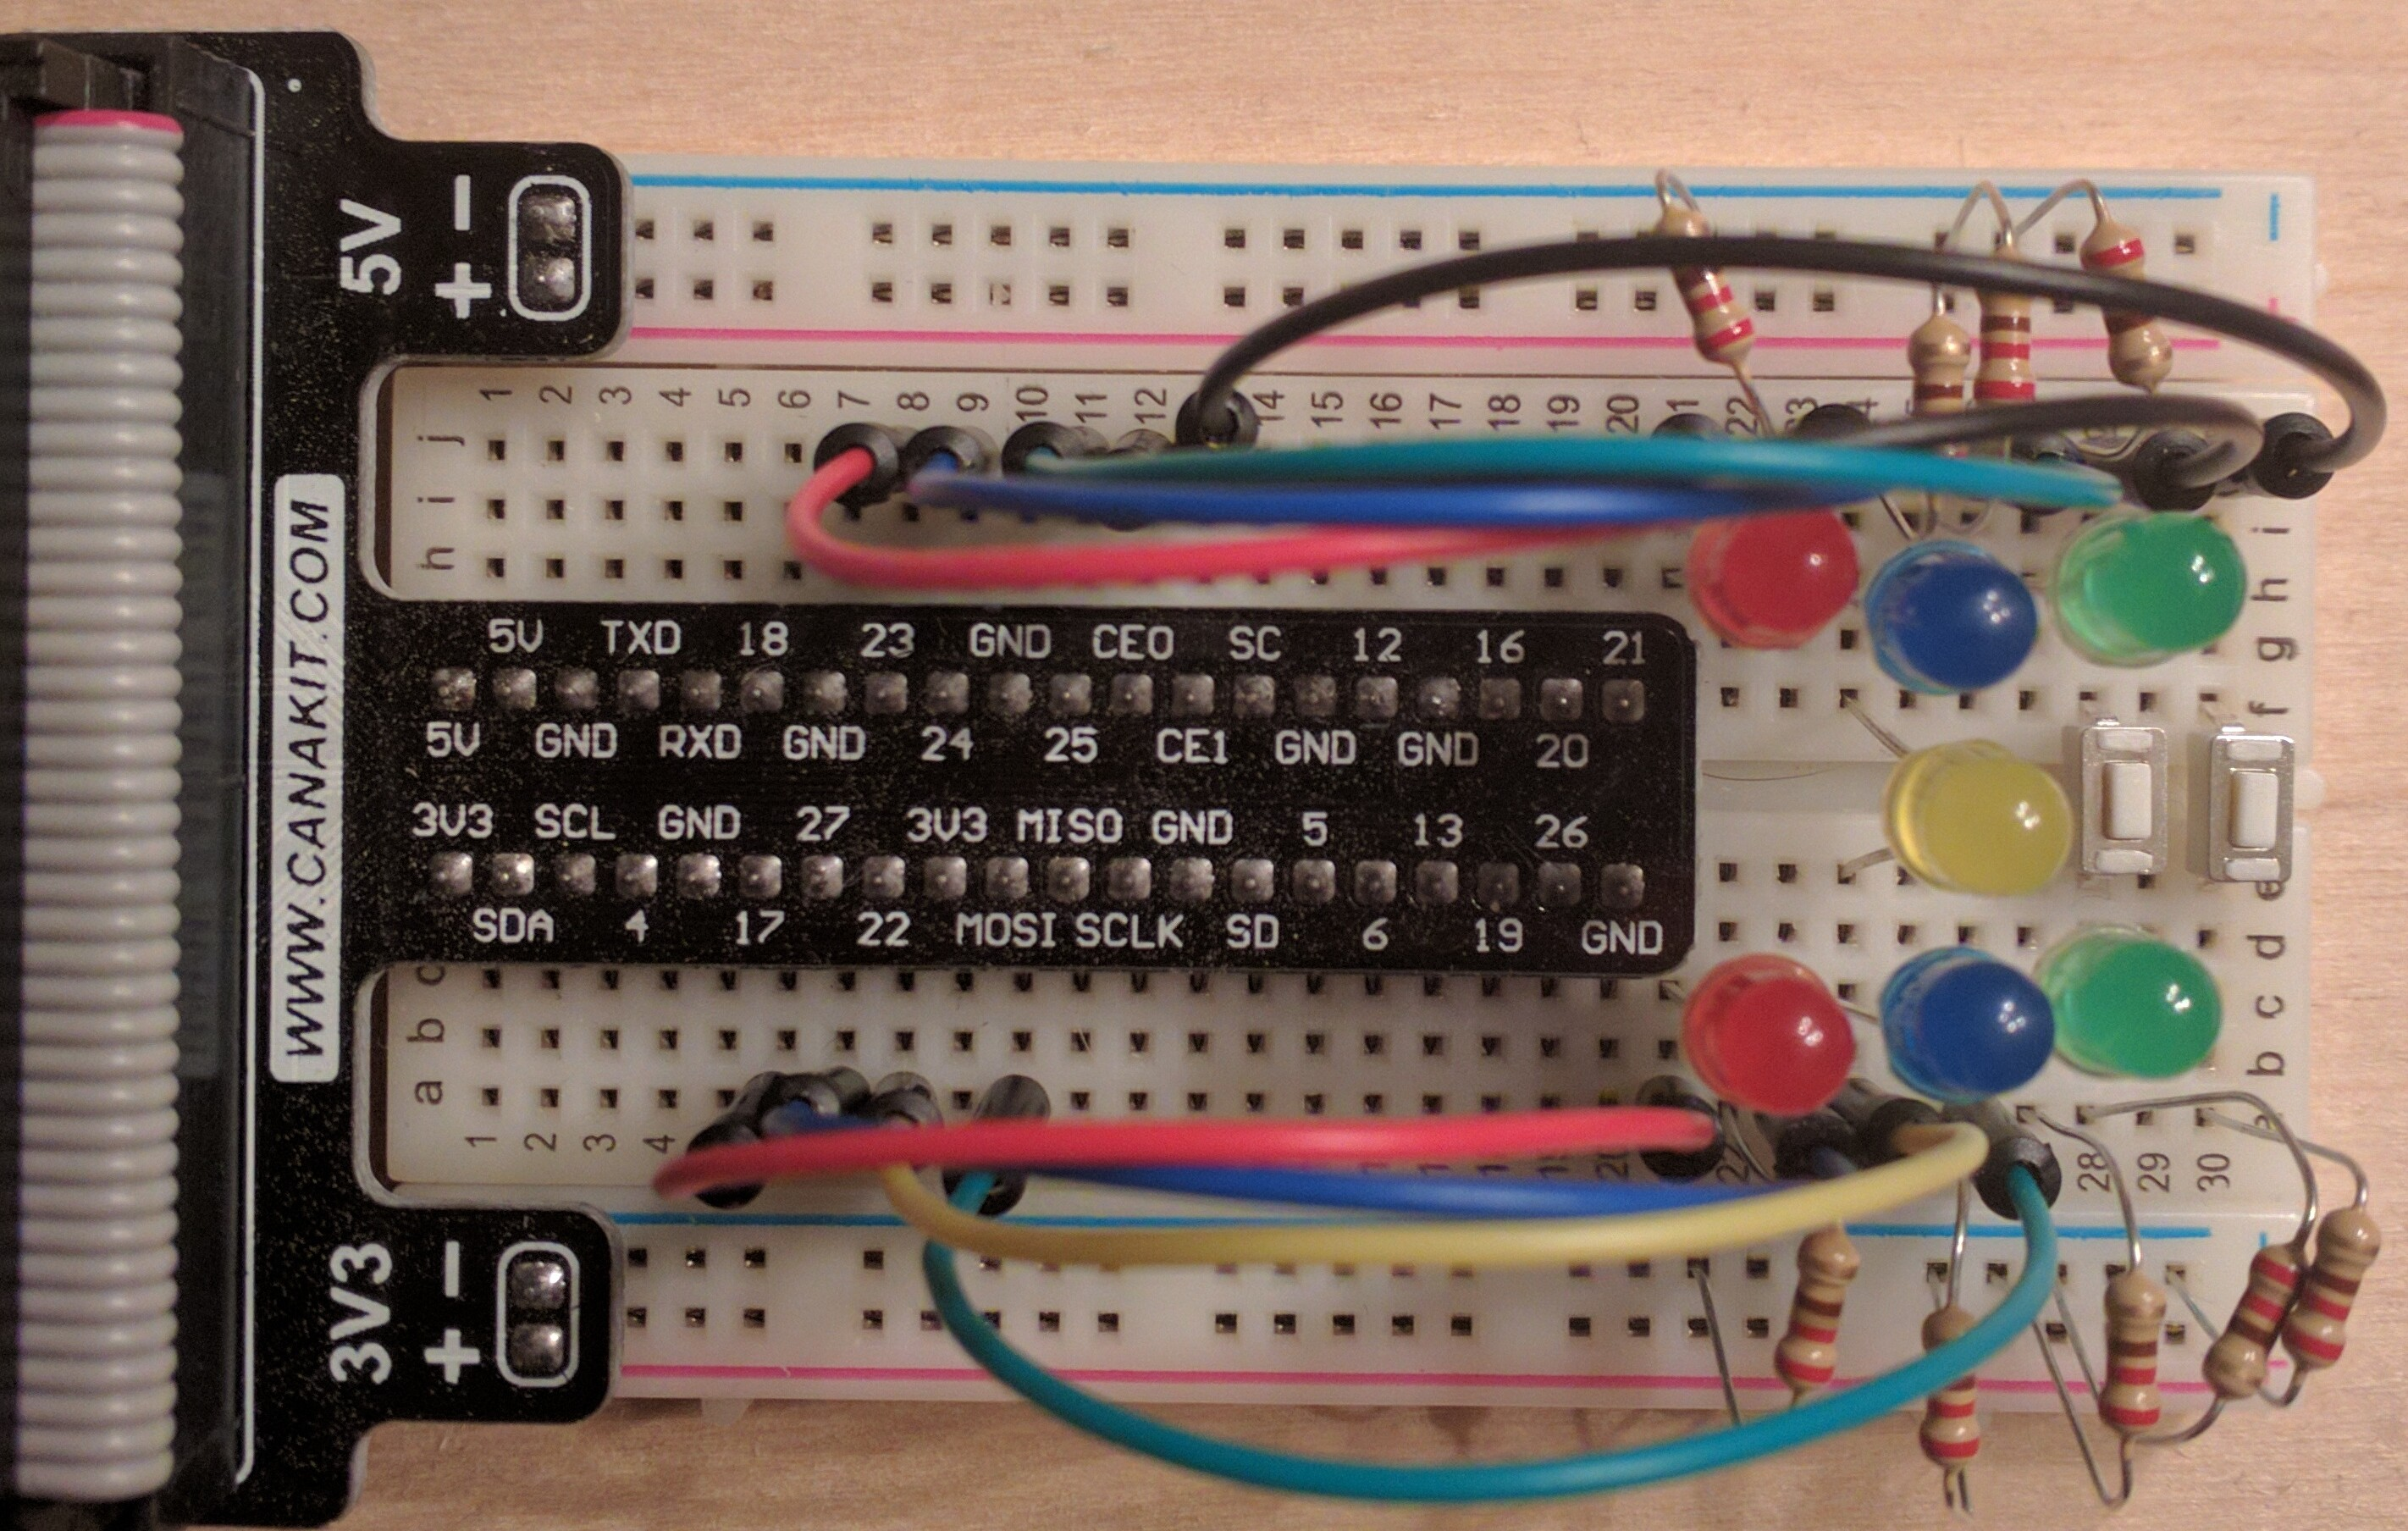
\includegraphics[height=2in]{pi_images/lab05images/PiLab05-DieLightPhoto.jpg}}
\afterfig

\newpage

\underline{GPIO Assignments}

\begin{center}
	\begin{tabular}{c | c | c}
		\hline
		\textbf{Type} & \textbf{GPIO} & \textbf{Description} \\ \hline
		Led & 0 & Upper Left LED\\ 
		\hline
		Led & 2 & Middle Left LED\\ 
		\hline
		Led & 12 & Lower Left LED\\ 
		\hline
		Led & 3 & Center LED\\ 
		\hline
		Led & 4 & Upper Right LED\\ 
		\hline
		Led & 5 & Middle Right LED\\ 
		\hline
		Led & 6 & Lower Right LED\\ 
		\hline
		Button & 10 & Upper Button (roll the die) \\ 
		\hline
		Button & 11 & Lower Button (end program) \\ 
		\hline	
	\end{tabular}
\end{center}

\vspace{10pt}

Start up your Pi and remember to start the \textbf{PiLib Server}. Bring up the Eclipse environment. Download and setup the PiLab05 project from the class website.

\underline{Run the Wiring Test}

Open the \textbf{\texttt{WiringTest}} program and run it. For information about wiring tests and common problems when testing your breadboard project please see the description on page \pageref{wiringTestDescription}.

\textbf{Program Implementation}

The project contains two source code files named \texttt{Die} and \texttt{DieExtraChallenge}. Start out by writing the code in the \texttt{Die} class.

\textit{Your program is to work as follows:}

When the user presses the upper button the die is rolled. The result of the die roll (a random number) should then be displayed using the LEDs. Here is how each of the six possible values should be displayed by the LEDs:

{\centering
	\beforefig
	\centerline{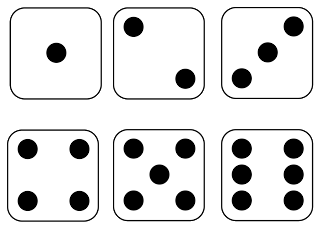
\includegraphics[height=1in]{pi_images/lab05images/DieFaces.png}}
	\afterfig
}

\begin{enumerate}
	\item The center LED lights up
	\item The 2 middle LEDs light up
	\item The upper right, the center, and lower left LEDs light up
	\item The 2 upper and 2 lower LEDs light up
	\item The 2 upper, center, and 2 lower green LEDs light up
	\item All left and right LEDs light up
\end{enumerate}

The upper button can then be pressed again to produce anther die roll value. This repeated use of the upper button may continue for any number of rolls. 

The lower button will end the program.

A video of what this lab might end up looking like when run is located at: \url{https://youtu.be/Us-4H5NqiHE}

\textit{Once you get your electronic die working, move onto part 2 of the lab.}

\section{Lab 5 - Part 2}

For this part of the lab, start out by copying your code from \texttt{Die} to \texttt{DieExtraChallenge}. Then make the following update to the operation of the \texttt{DieExtraChallenge} class.

Add a feature that displays random die values (or consecutive values) until the user presses the upper button to get a roll value. Pressing the upper button again would return to displaying the random values until the upper button is pressed again to display a random roll.

The lower button will still exit the program.

A video of what part 2 of the lab might end up looking like when run is located at: \url{https://youtu.be/eRAkxTZcGa0}
 
\textbf{End of Lab}
  
This concludes lab 5. You generated random values and controlled a set of LEDs to format a electronic die.

\textbf{Remember to submit your completed lab using the process defined by your instructor.}

{\centering
	\beforefig
	\centerline{
\includegraphics[height=1in]{pi_images/stop_sign_clip_art_16252.jpg}}
	\afterfig
}

\newpage

\section{Lab 6 - Part 1}

\textbf{Learning Goals}

\begin{enumerate}
	\item Keep track of LEDs and buttons
	\item Learn how to use buttons for multiple purposes
\end{enumerate}

\textbf{Overview}

Create a circuit that has 2 LEDs and 2 buttons. Write a game where the user tries to guess which LED will light up. After the user guesses the computer displays the correct answer.

\textbf{Breadboard Configuration}

\underline{Wiring Depiction}

\beforefig
\centerline{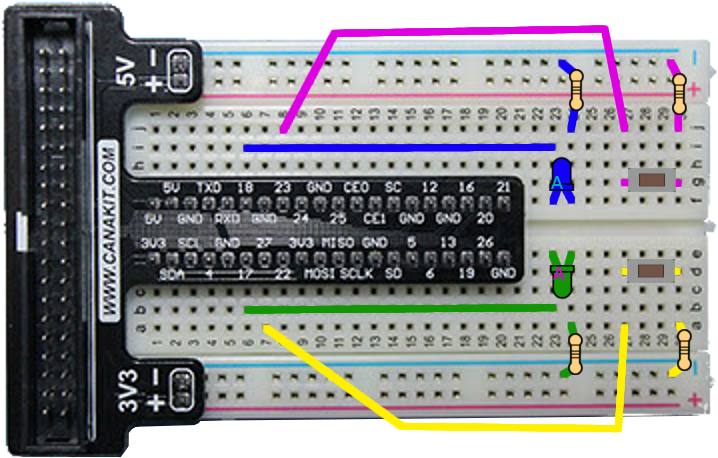
\includegraphics[height=2in]{pi_images/lab06images/PiLab06-GuessingGame.png}}
\afterfig

\underline{Wiring Steps}

\textbf{Remember, your Pi must be disconnected from a power source while wiring the circuit.}

\begin{enumerate}
	\item Insert a button into holes \textbf{d27} and \textbf{d30}
	\item Insert a button into holes \textbf{g27} and \textbf{g30}
	
	\item Insert the anode of an LED into hole \textbf{e23} the cathode into hole \textbf{e24}
	\item Insert the anode of an LED into hole \textbf{f23} the cathode into hole \textbf{f24}
	
	\item Insert a jumper from hole \textbf{b6} to hole \textbf{b23}
	\item Insert a jumper from hole \textbf{a7} to hole \textbf{a27}
	\item Insert a jumper from hole \textbf{i6} to hole \textbf{i23}	
	\item Insert a jumper from hole \textbf{j8} to hole \textbf{j27}

	\item Insert a resistor from hole \textbf{a24} to a \textbf{3V3--} hole adjacent to row 24
	\item Insert a resistor from hole \textbf{a30} to a \textbf{3V3--} hole adjacent to row 30
	\item Insert a resistor from hole \textbf{j24} to a \textbf{5V--} hole adjacent to row 24
	\item Insert a resistor from hole \textbf{j30} to a \textbf{5V--} hole adjacent to row 30
	
	\item If your ribbon cable is not connected do so now.
\end{enumerate}

\underline{Completed Breadboard Picture}

\beforefig
\centerline{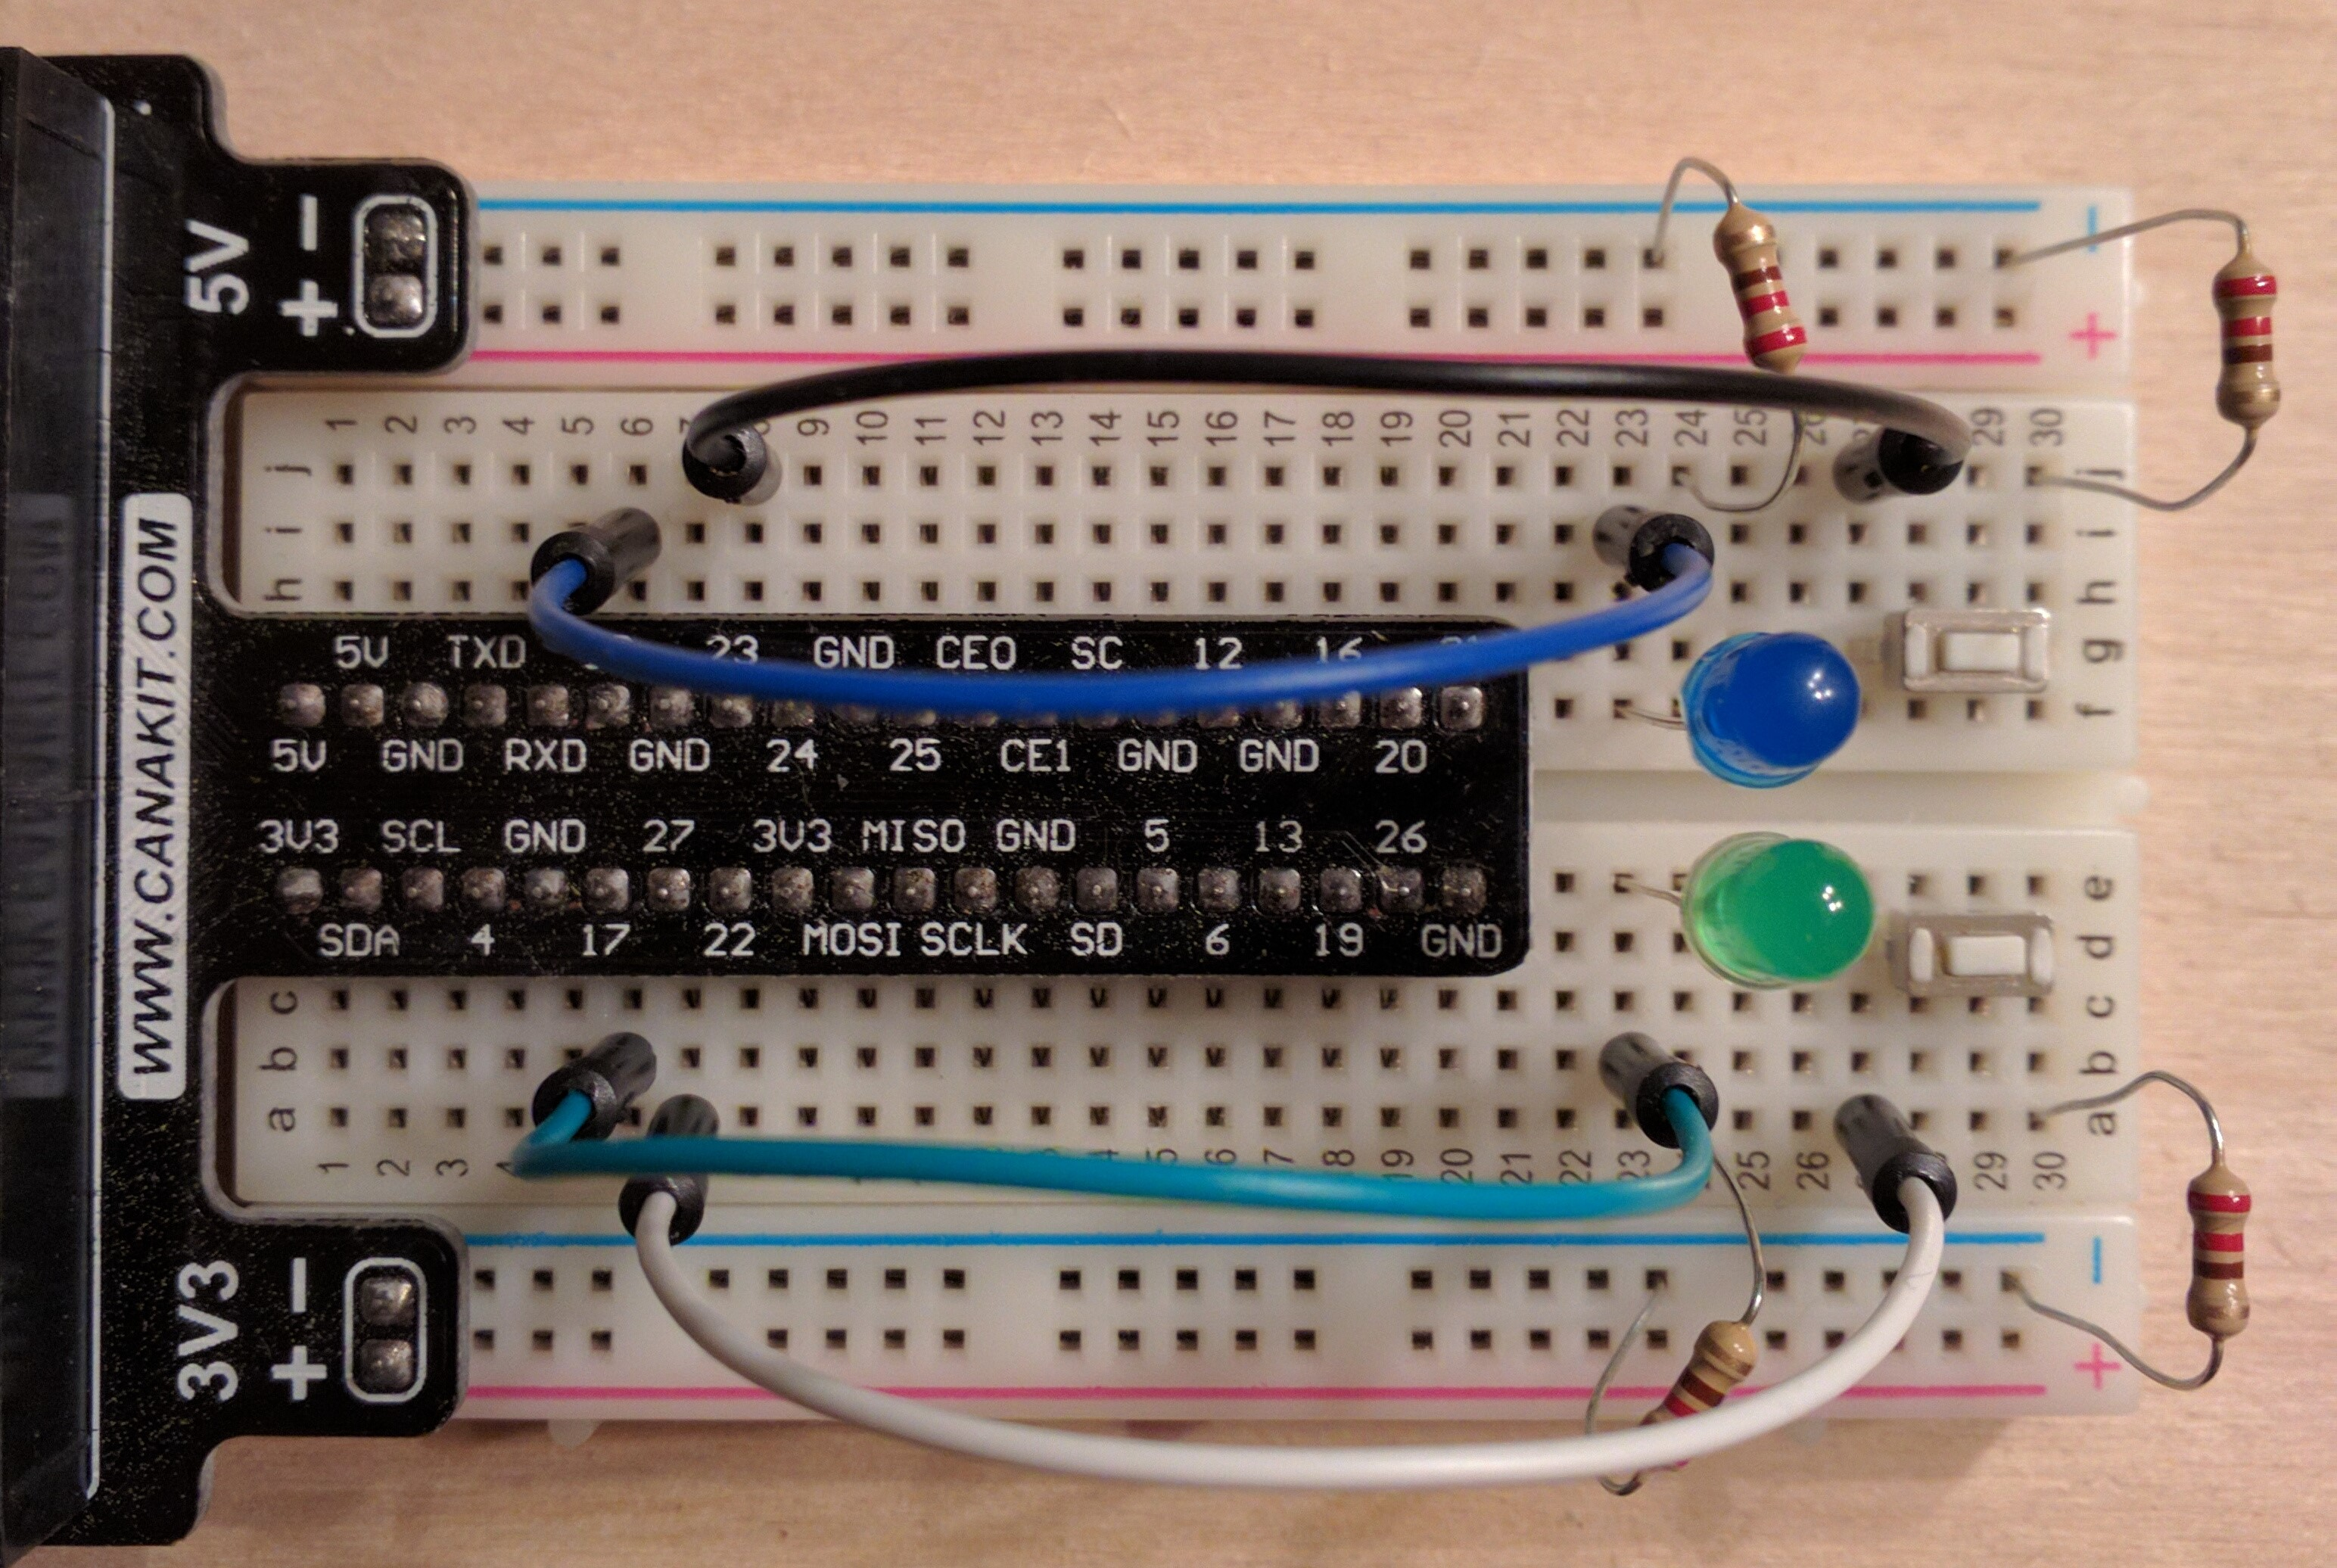
\includegraphics[height=2in]{pi_images/lab06images/PiLab06-GuessingGamePhoto.jpg}}
\afterfig

\underline{GPIO Assignments}

\begin{center}
	\begin{tabular}{c | c | c}
		\hline
		\textbf{Type} & \textbf{GPIO} & \textbf{Description} \\ \hline
		Led & 0 & Left LED \\ 
		\hline
		Led & 1 & Right LED \\ 
		\hline
		Button & 2 & Left Button \\ 
		\hline
		Button & 4 & Right Button \\ 
		\hline	
	\end{tabular}
\end{center}

\vspace{10pt}

Start up your Pi and remember to start the \textbf{PiLib Server}. Bring up the Eclipse environment. Download and setup the PiLab06 project from the class website.

\underline{Run the Wiring Test}

Open the \textbf{\texttt{WiringTest}} program and run it. For information about wiring tests and common problems when testing your breadboard project please see the description on page \pageref{wiringTestDescription}.

\textbf{Program Implementation}

The project contains two source code files named \texttt{GuessingGame} and \texttt{GuessingGameExtraChallenge}. Start out by coding the \texttt{GuessingGame} class.

\textit{Your program is to work as follows:}

On startup the two LEDs will alternate lighting up, signaling the program is ready for user input. The user then presses one of the two buttons, indicating which LED they think the computer will choose. The computer then displays the LED that it picked. If the user picked correctly the LED will stay on solid. If the user picked incorrectly the LED will flash. Pressing either button will exit the program.

A video of what this lab might end up looking like when run is located at: \url{https://youtu.be/jsREOiKE2Aw}

\texttt{Once you have your guessing game working, move onto part 2 of the lab.}

\section{Lab 6 - Part 2}

For this part of the lab, start out by copying your code from \texttt{GuessingGame} to \texttt{GuessingGameExtraChallenge}. Then make the following update to the operation of the \texttt{GuessingGameExtraChallenge} class.

In this version you will allow the user to keep playing the game until they choose to have it end. Like your initial version, the program starts out waiting for the user to guess which light the computer will choose. Once the computer displays the result, the left-hand button allows the user to play again. When the button is pushed the two LEDs will alternate lighting up as they did on program startup and it will wait for the user to guess again.

If the user presses the right-hand button after their guess, the program will exit.

A video of what this lab might end up looking like when run is located at: \url{https://youtu.be/l13m_5HtuLc}

\textbf{End of Lab}

This concludes lab 6. You created a guessing game that the user can play against the computer.

\textbf{Remember to submit your completed lab using the process defined by your instructor.}

{\centering
	\beforefig
	\centerline{
\includegraphics[height=1in]{pi_images/stop_sign_clip_art_16252.jpg}}
	\afterfig
}

\newpage

\section{Lab 7 - Part 1}

\textbf{Learning Goals}

\begin{enumerate}
	\item Work with binary numbers and represent them with LEDs
	\item See the effects of bitshifting
\end{enumerate}

\textbf{Overview}

Create a circuit that has 5 LEDs and 2 buttons. Write a program that allows the user to add or subtract one from a value which is then displayed (in binary) by the set of LEDs.

\textbf{Breadboard Configuration}

\underline{Wiring Depiction}

\beforefig
\centerline{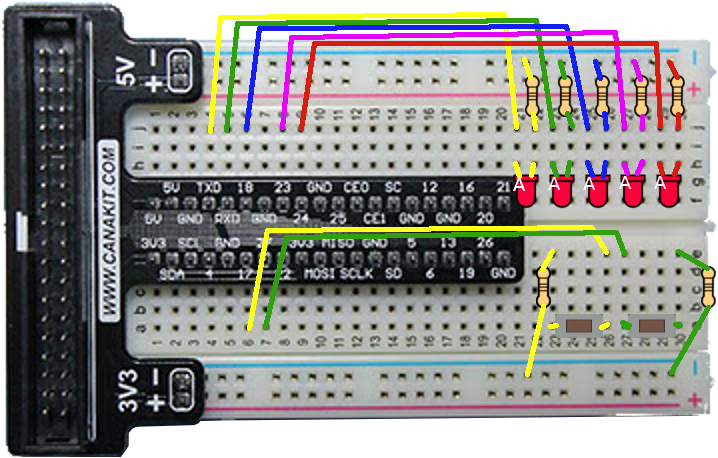
\includegraphics[height=2in]{pi_images/lab07images/PiLab07-Binary.png}}
\afterfig

\underline{Wiring Steps}

\textbf{Remember, your Pi must be disconnected from a power source while wiring the circuit.}

\begin{enumerate}
%	\item Insert a button into holes \textbf{c27} and \textbf{c30}
%	\item Insert a button into holes \textbf{h27} and \textbf{h30}
	\item Insert a button into holes \textbf{a23} and \textbf{a26}
    \item Insert a button into holes \textbf{a27} and \textbf{a30}
	
%	\item Insert the anode of an LED into hole \textbf{b21} the cathode into hole \textbf{b22}
%	\item Insert the anode of an LED into hole \textbf{c23} the cathode into hole \textbf{c24}
%	\item Insert the anode of an LED into hole \textbf{d25} the cathode into hole \textbf{d26}
%	\item Insert the anode of an LED into hole \textbf{e28} the cathode into hole \textbf{e29}
%	\item Insert the anode of an LED into hole \textbf{i21} the cathode into hole \textbf{i22}
%	\item Insert the anode of an LED into hole \textbf{h23} the cathode into hole \textbf{h24}
%	\item Insert the anode of an LED into hole \textbf{g25} the cathode into hole \textbf{g26}
%	\item Insert the anode of an LED into hole \textbf{f28} the cathode into hole \textbf{f29}

	\item Insert the anode of an LED into hole \textbf{h21} the cathode into hole \textbf{h22}
    \item Insert the anode of an LED into hole \textbf{h23} the cathode into hole \textbf{c24}
    \item Insert the anode of an LED into hole \textbf{h25} the cathode into hole \textbf{h26}
    \item Insert the anode of an LED into hole \textbf{h27} the cathode into hole \textbf{h28}
    \item Insert the anode of an LED into hole \textbf{h29} the cathode into hole \textbf{h30}
					
%	\item Insert a jumper from hole \textbf{a6} to hole \textbf{a21}
%	\item Insert a jumper from hole \textbf{a7} to hole \textbf{a23}
%	\item Insert a jumper from hole \textbf{a8} to hole \textbf{a25}	
%	\item Insert a jumper from hole \textbf{a10} to hole \textbf{a27}
%	\item Insert a jumper from hole \textbf{a11} to hole \textbf{a28}

%	\item Insert a jumper from hole \textbf{j4} to hole \textbf{j21}
%	\item Insert a jumper from hole \textbf{j5} to hole \textbf{j23}
%	\item Insert a jumper from hole \textbf{j6} to hole \textbf{j25}	
%	\item Insert a jumper from hole \textbf{j8} to hole \textbf{j27}
%	\item Insert a jumper from hole \textbf{j9} to hole \textbf{j28}

    \item Insert a jumper from hole \textbf{a6} to hole \textbf{e26}
    \item Insert a jumper from hole \textbf{a7} to hole \textbf{e27}
	\item Insert a jumper from hole \textbf{j4} to hole \textbf{j21}
    \item Insert a jumper from hole \textbf{j5} to hole \textbf{j23}
    \item Insert a jumper from hole \textbf{j6} to hole \textbf{j25}	
    \item Insert a jumper from hole \textbf{j8} to hole \textbf{j27}
    \item Insert a jumper from hole \textbf{j9} to hole \textbf{j29}
		
%	\item Insert a resistor from hole \textbf{a22} to a \textbf{3V3--} hole adjacent to row 22
%	\item Insert a resistor from hole \textbf{a24} to a \textbf{3V3--} hole adjacent to row 24
%	\item Insert a resistor from hole \textbf{a26} to a \textbf{3V3--} hole adjacent to row 26
%	\item Insert a resistor from hole \textbf{a29} to a \textbf{3V3--} hole adjacent to row 29
%	\item Insert a resistor from hole \textbf{a30} to a \textbf{3V3--} hole adjacent to row 30	
%	\item Insert a resistor from hole \textbf{j22} to a \textbf{5V--} hole adjacent to row 22
%	\item Insert a resistor from hole \textbf{j24} to a \textbf{5V--} hole adjacent to row 24
%	\item Insert a resistor from hole \textbf{j26} to a \textbf{5V--} hole adjacent to row 26
%	\item Insert a resistor from hole \textbf{j29} to a \textbf{5V--} hole adjacent to row 29
%	\item Insert a resistor from hole \textbf{j30} to a \textbf{5V--} hole adjacent to row 30		
	
	
	\item Insert a resistor from hole \textbf{e23} to a \textbf{3V3--} hole adjacent to row 23
	\item Insert a resistor from hole \textbf{e30} to a \textbf{3V3--} hole adjacent to row 30
	\item Insert a resistor from hole \textbf{j22} to a \textbf{5V--} hole adjacent to row 22
	\item Insert a resistor from hole \textbf{j24} to a \textbf{5V--} hole adjacent to row 24
	\item Insert a resistor from hole \textbf{j26} to a \textbf{5V--} hole adjacent to row 26
	\item Insert a resistor from hole \textbf{j28} to a \textbf{5V--} hole adjacent to row 28
	\item Insert a resistor from hole \textbf{j30} to a \textbf{5V--} hole adjacent to row 30		
	
	\item If your ribbon cable is not connected do so now.
\end{enumerate}

%\newpage

\underline{Completed Breadboard Picture}

\beforefig
\centerline{\includegraphics[height=2in]{pi_images/lab07images/PiLab07-BinaryPhoto.jpg}}
\afterfig

\underline{GPIO Assignments}

\begin{center}
	\begin{tabular}{c | c | c}
%		\hline
%		\textbf{Type} & \textbf{GPIO} & \textbf{Description} \\ \hline
%		BinaryLed & 15 & Right-most LED (2\textsuperscript{0} $\equiv$ 1) \\ 
%		\hline
%		BinaryLed & 16 & Second-to-the-right LED (2\textsuperscript{1} $\equiv$ 2) \\ 
%		\hline
%		BinaryLed & 1 & Third-to-the-right LED (2\textsuperscript{2} $\equiv$ 4) \\ 
%		\hline
%		BinaryLed & 5 & Fourth-to-the-right LED (2\textsuperscript{3} $\equiv$ 8) \\ 
%		\hline
%		BinaryLed & 13 & Fourth-to-the-left LED (2\textsuperscript{4} $\equiv$ 16) \\ 
%		\hline
%		BinaryLed & 3 & Third-to-the-left LED (2\textsuperscript{5} $\equiv$ 32) \\ 
%		\hline
%		BinaryLed & 2 & Second-to-the-left LED (2\textsuperscript{6} $\equiv$ 64) \\ 
%		\hline
%		BinaryLed & 0 & Left-most LED (2\textsuperscript{7} $\equiv$ 128) \\ 
		\hline
		\textbf{Type} & \textbf{GPIO} & \textbf{Description} \\ \hline
		BinaryLed & 5 & Right-most LED (2\textsuperscript{0} $\equiv$ 1) \\ 
		\hline
		BinaryLed & 4 & Second-to-the-right LED (2\textsuperscript{1} $\equiv$ 2) \\ 
		\hline
		BinaryLed & 1 & Third-to-the-right LED (2\textsuperscript{2} $\equiv$ 4) \\ 
		\hline
		BinaryLed & 16 & Fourth-to-the-right LED (2\textsuperscript{3} $\equiv$ 8) \\ 
		\hline
		BinaryLed & 15 & Left-most LED (2\textsuperscript{4} $\equiv$ 16) \\ 
		\hline
		Button & 0 & Left Button (decrement)\\ 
		\hline
		Button & 2 & Right Button (increment)\\ 
		\hline	
	\end{tabular}
\end{center}

\vspace{10pt}

Start up your Pi and remember to start the \textbf{PiLib Server}. Bring up the Eclipse environment. Download and setup the PiLab07 project from the class website.

\underline{Run the Wiring Test}

Open the \textbf{\texttt{WiringTest}} program and run it. For information about wiring tests and common problems when testing your breadboard project please see the description on page \pageref{wiringTestDescription}.

%\newpage 

\textbf{Program Implementation}

The project contains two source code files named \texttt{BinaryNumbers} and \texttt{BinaryNumbersBitShift}. Start out by coding the \texttt{BinaryNumbers} class.

A couple of notes as you get started coding this lab:

\begin{enumerate}
	\item The LEDs are displaying a binary number with the \textbf{least significant bit (LSB) to the right.} \textit{This means that you'll need to create the BinaryLed instances (e.g. using the \texttt{BinaryLed} class) from the right-most LED (representing 2\textsuperscript{0}) to the left-most LED (representing 2\textsuperscript{4}).}
	\item The \texttt{Widget} class contains the method \texttt{setBinaryValue()} which takes the integer value to be displayed as its parameter. For example the call \texttt{Widget.setBinaryValue(22)} will cause the LEDs mapped to \texttt{BinaryLed} instances to be turned on and off to match the value \texttt{10110}, which is decimal 22 in binary.
\end{enumerate}

\textit{Your program is to work as follows:}

On startup the LEDs will display the number 1 (e.g. the right-most LED will be illuminated). Pressing the left-hand button will subtract one from the current value and update the LEDs while pressing the right-hand button will add 1 to the value and update the LEDs. The program should end if the value becomes either -1 or 32.

\textit{You may want to display the value on the console as well so that you can verify that the value displayed by the LEDs agrees with the value you are calculating.}

A video of what this lab might end up looking like when run is located at: \url{https://youtu.be/FA42EsYA1LY}

\texttt{Once you have your binary counting program working, move onto part 2 of the lab.}

\newpage

\section{Lab 7 - Part 2}

For this part of the lab, start out by copying your code from \texttt{BinaryNumbers} to \texttt{BinaryNumbersBitShifting}. Then make the following update to the operation of the \texttt{BinaryNumbersBitShifting} class.

In this version you will interpret the left-hand button as a left-shift request and the right-hand button as a right-shift request. Your program may use signed (\textgreater\textgreater) or unsigned right-shift (\textgreater\textgreater\textgreater) at your discretion. When the program starts, the user should be asked to enter a number (using the keyboard) between 1 and 31. The LEDs should initially display the entered value and then bit-shifting should be used to update that value. The program is to  exit if the bit-shifting operation changes the value to 0 (or less) or 32 (or more).

\textbf{Note: you are to use the shift operators (\textless\textless, \textgreater\textgreater, \textgreater\textgreater\textgreater), not the multiplication and division operators.}

\textit{You may want to display the value on the console as well so that you can verify that the value displayed by the LEDs agrees with the value you are calculating.}

A video of what this lab might end up looking like when run is located at: \url{https://youtu.be/7e-3w8dlngI}

\textbf{End of Lab}

This concludes lab 7. You displayed numbers as binary values and carried out bit-shifting.

\textbf{Remember to submit your completed lab using the process defined by your instructor.}

{\centering
	\beforefig
	\centerline{
\includegraphics[height=1in]{pi_images/stop_sign_clip_art_16252.jpg}}
	\afterfig
}

